\newpage
\section{Hardware implementation and module tests}
This section details the different hardware modules used by the system, such as the voltage regulators, the controller, the GPS receiver, and more. Furthermore, each has a short description of how the unit was tested.

\subsection{Voltage regulators}
As mentioned in the \nameref{sec:hardware_design} section, two voltage regulators are needed, both of them 5~V.
LM2596 was chosen, and to get them to work, all that has to be done is to supply them with a voltage a bit higher then the expected output voltage. In this case the output voltage we want is 5 V, and the battery voltage is 8.4 V nominal, which is high enough to supply the regulators. The voltage regulator just has to be adjusted to output 5 V. 

\begin{figure}[H]
	\centering
	\subfloat[Voltage output of a voltage regulator] {
		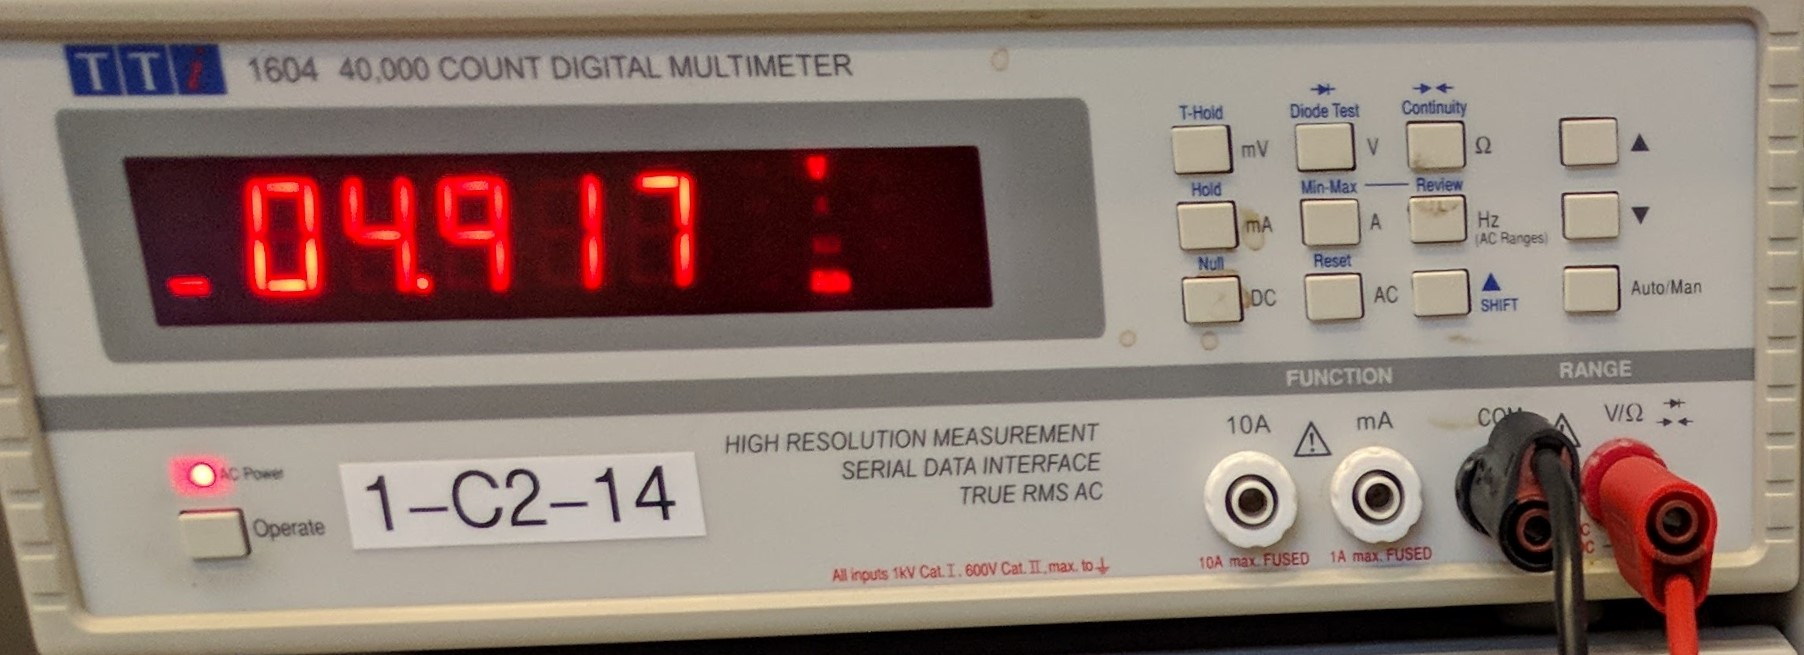
\includegraphics[width=0.32\textwidth]{Images/Implementation/stepdown_adjustment}
		\label{fig:stepdown_output_voltage}
	}
	\hfill
	\subfloat[Measurement setup]{
		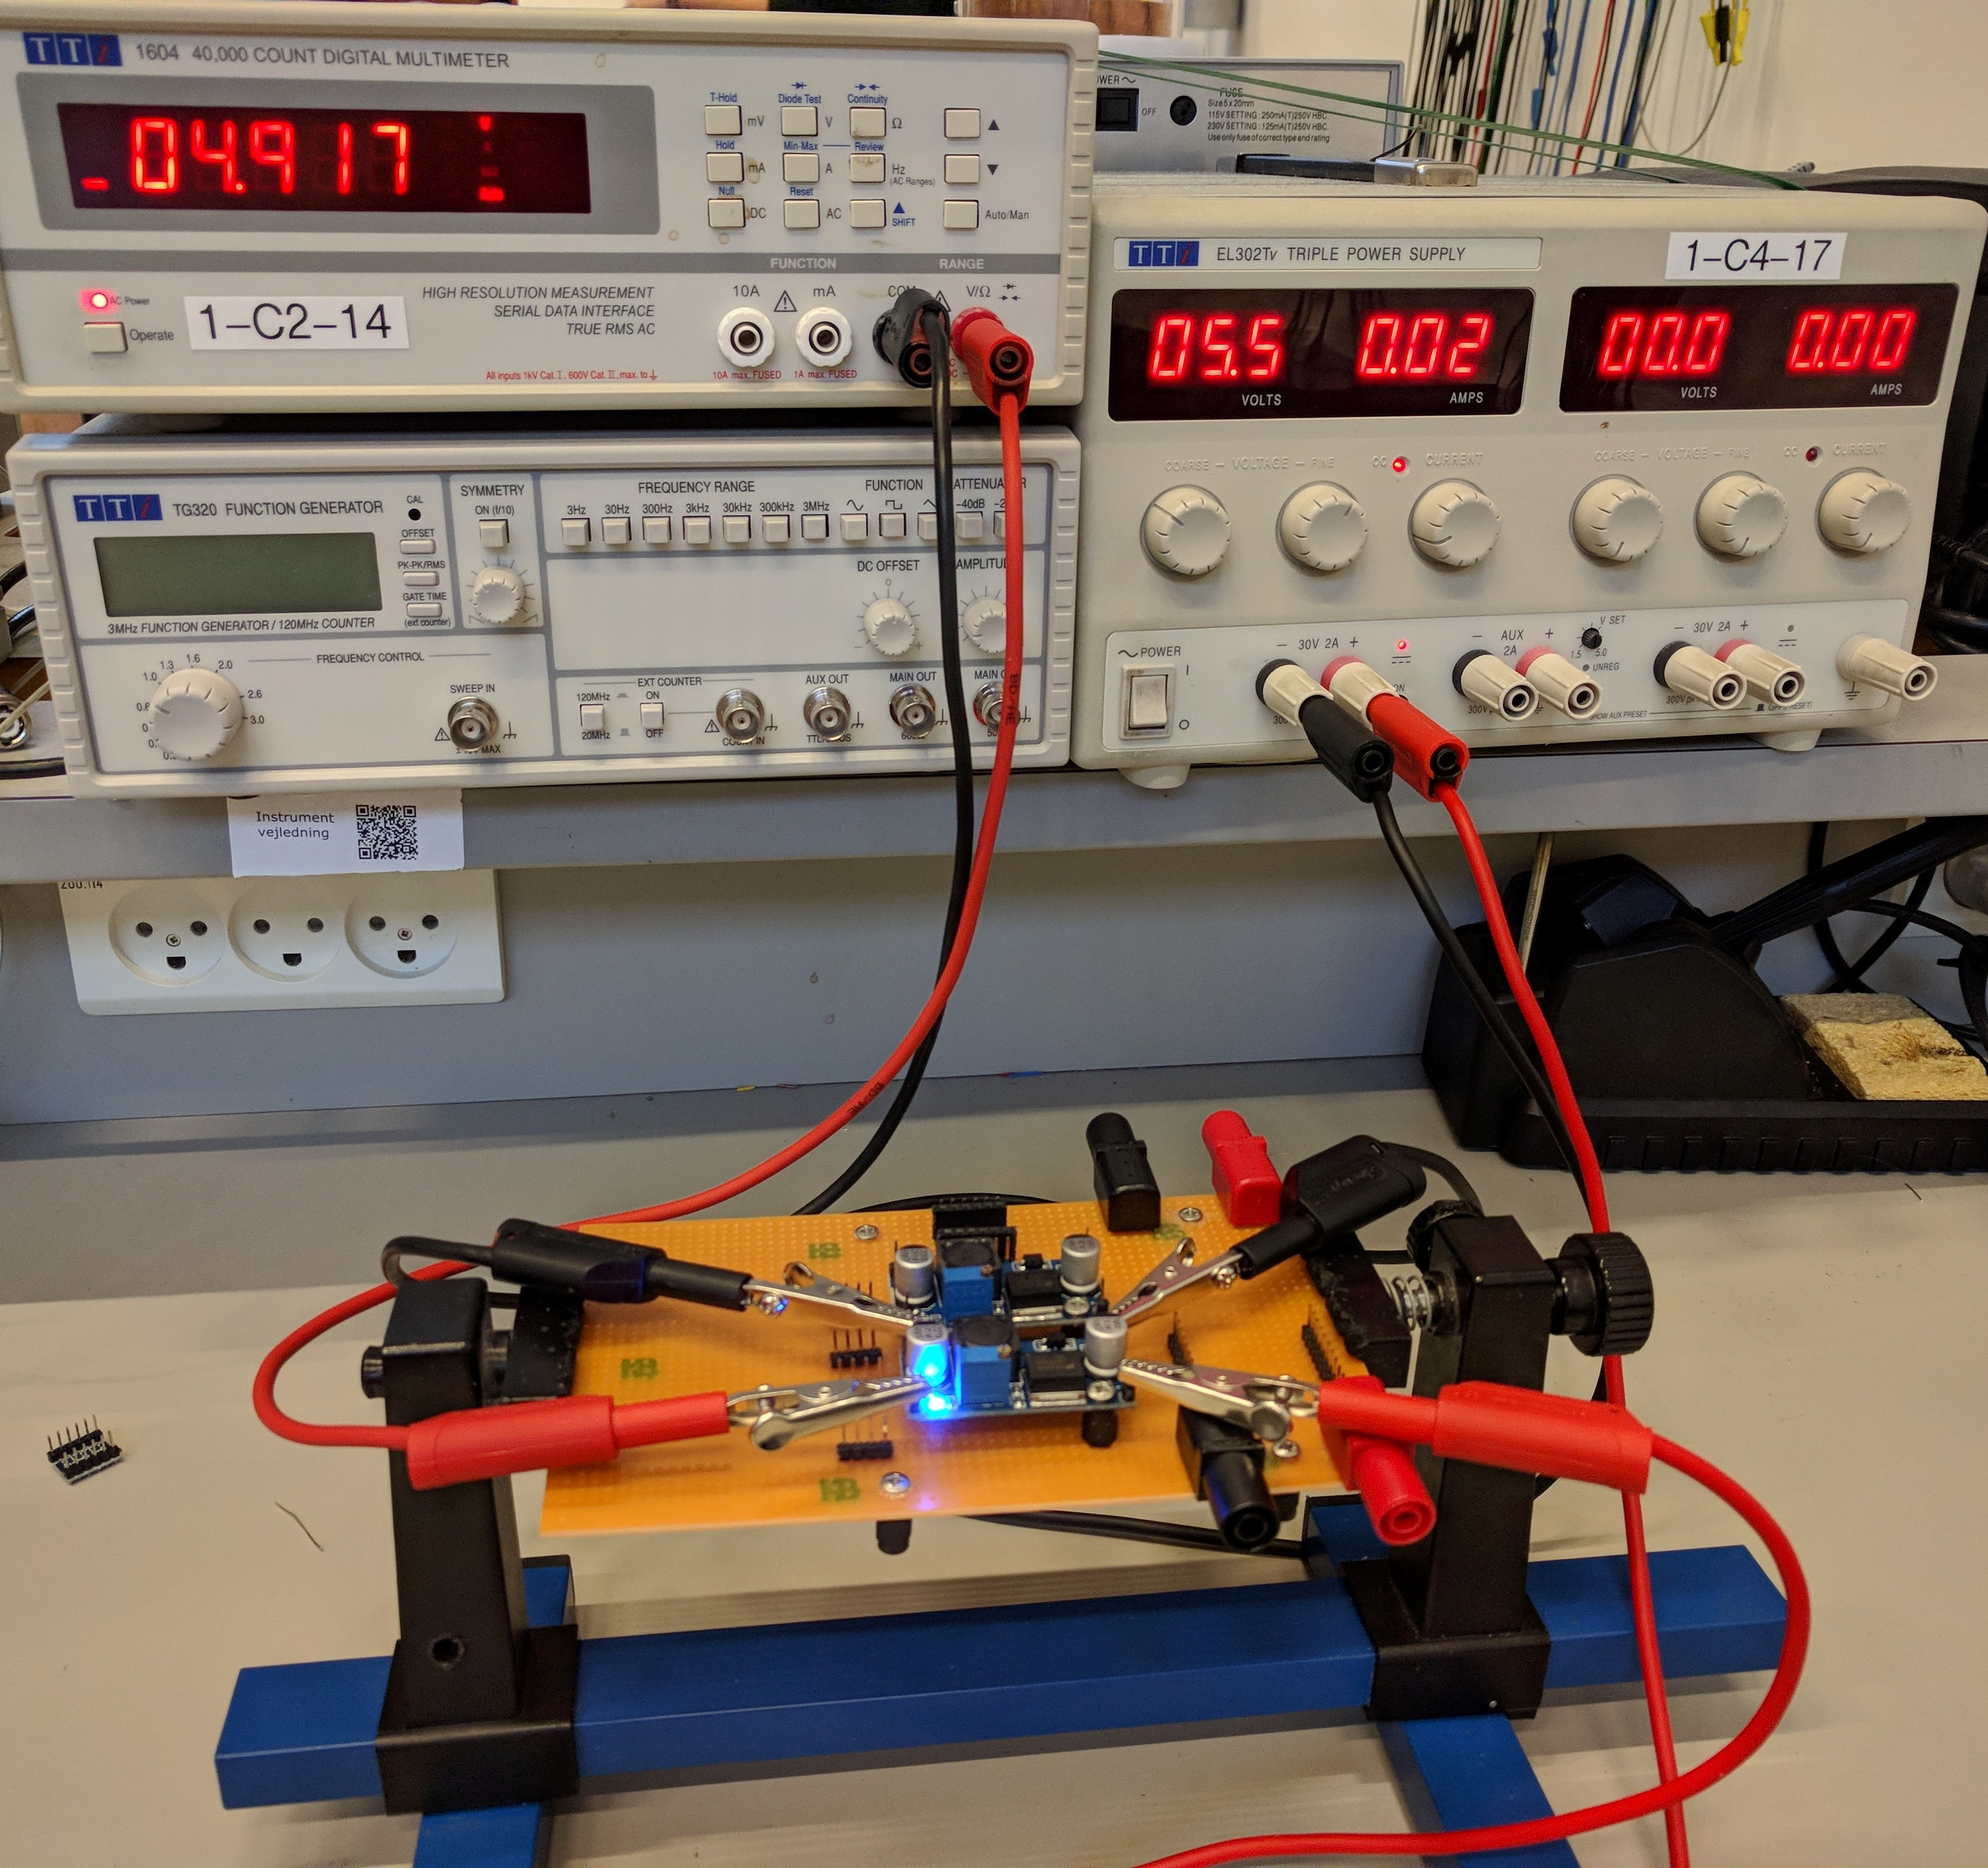
\includegraphics[width=0.32\textwidth]{Images/Implementation/stepdown_setup}
		\label{fig:stepdown_setup}
	}
	\hfill
	\subfloat[Current draw of a regulators]{
		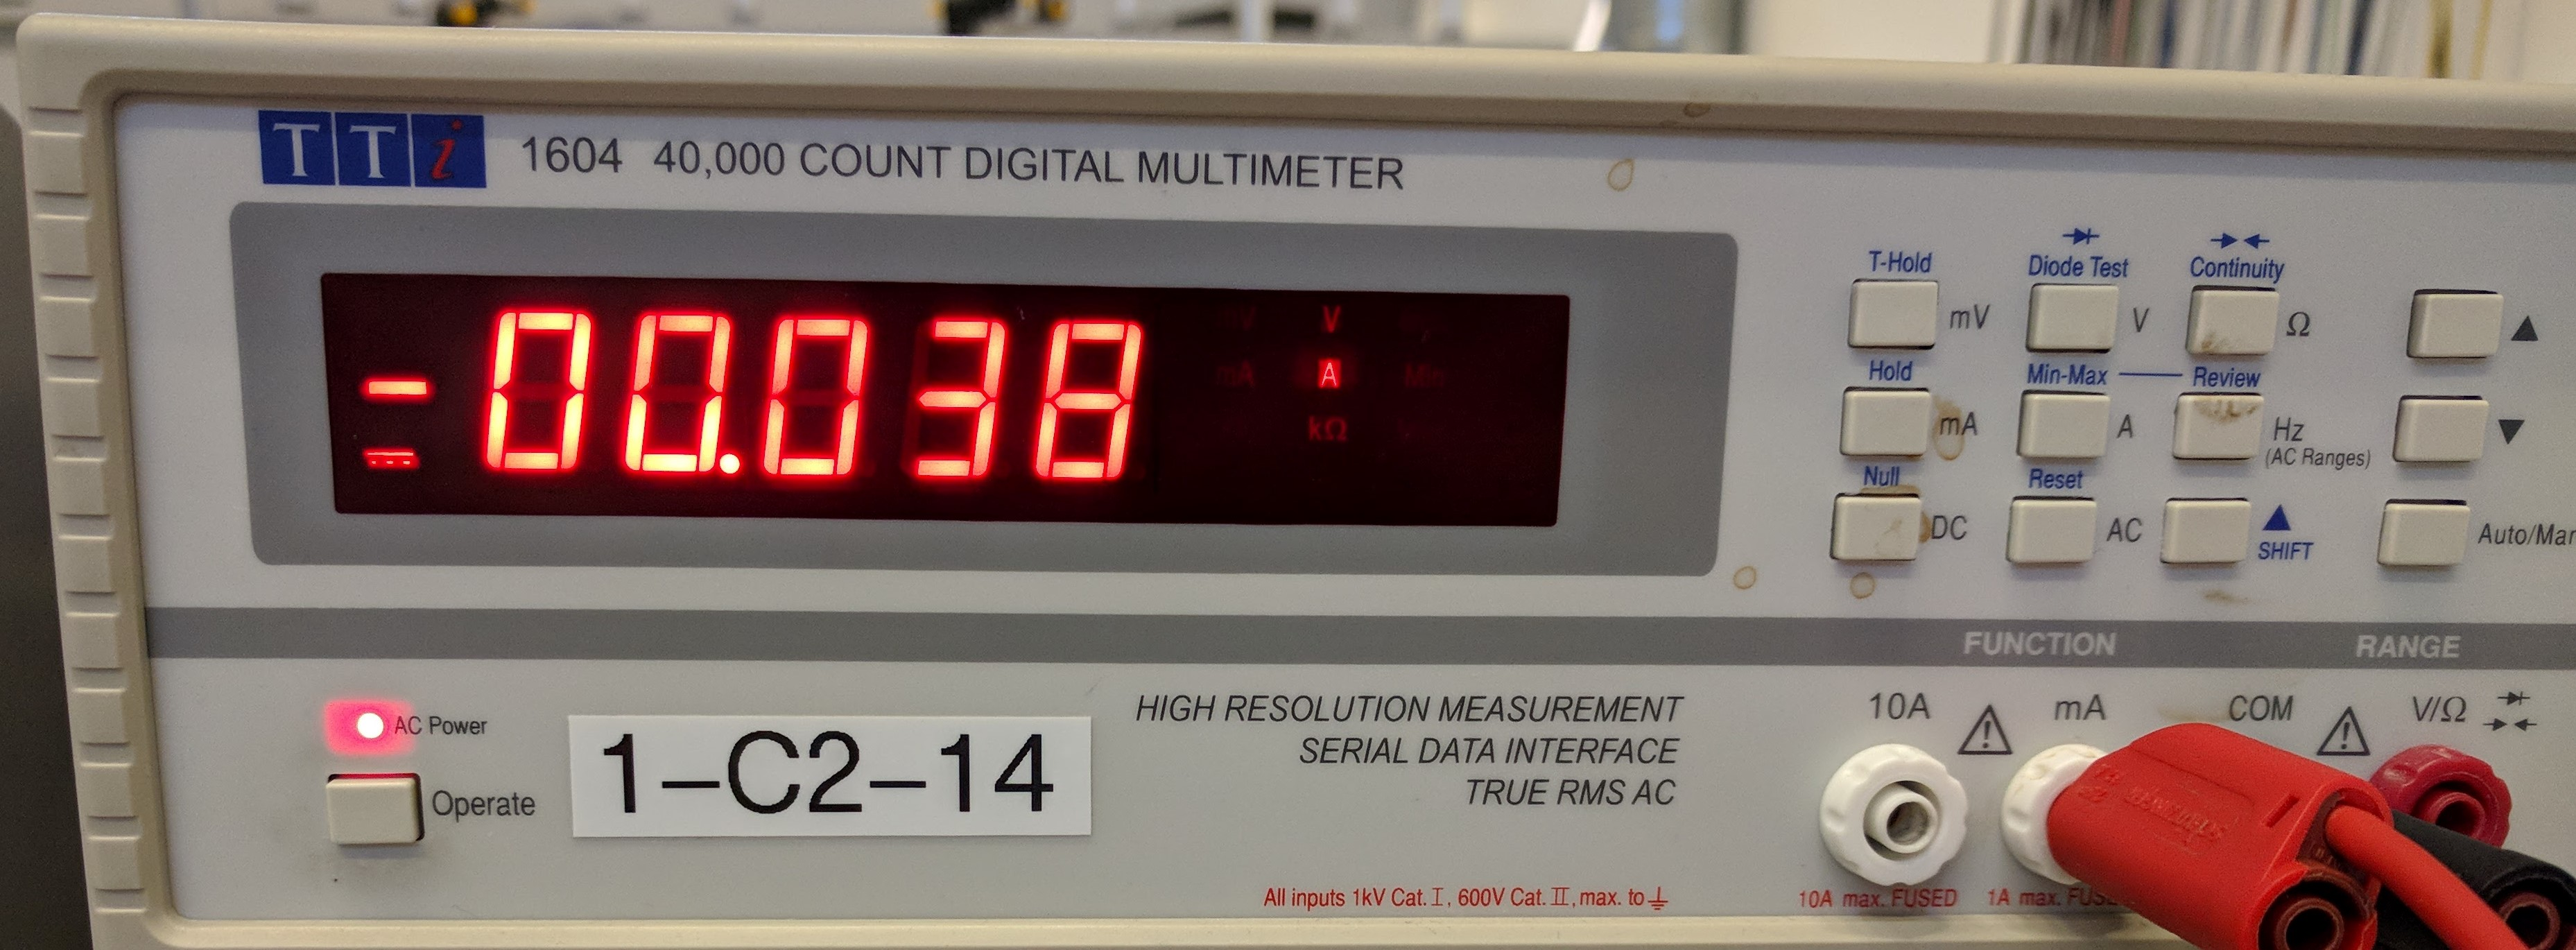
\includegraphics[width=0.32\textwidth]{Images/Implementation/stepdown_current_draw}
		\label{fig:stepdown_currentdraw}
	}
	\caption{Voltage and current draw tests}
\end{figure}

To test the voltage regulators they were adjusted to about 5 V and the input voltage was to only 5.5 V, and as seen on figure~\ref{fig:stepdown_output_voltage} the output is just under 5 V.  The current draw of a voltage regulator was also measured, to about 38 mA, as seen on figure~\ref{fig:stepdown_currentdraw}.

\subsection{Servo}
The servo in the system, was a consequence of the boat chosen.  So to test the servo, a frequency generator was set to a 50 Hz square wave and 7\% or about 1.2 ms period. This duty cycle is with in the servo PWM range of 500 µs to 2500µs. The frequency generator settings can be seen on figure~\ref{fig:servopwmtest}. The servo needs a 5 V power supply, the 5 V step down regulator and the battery was used. Now when then PWM signal is applied, the servo should turn to some position and try to hold it. That is in fact what happens. 

\begin{figure}[h]
\centering
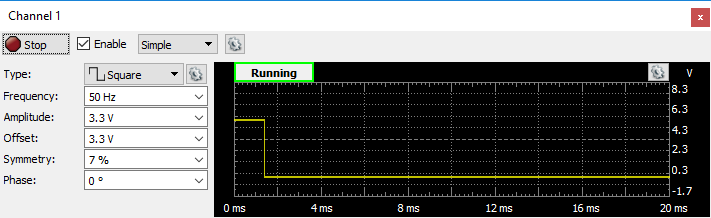
\includegraphics[width=0.7\linewidth]{Images/Implementation/Servo_PWM_test}
\caption{Frequency generator setup}
\label{fig:servopwmtest}
\end{figure}

\subsection{Motor Controller}
\label{sec:motor_controller}
The motor controller that was chosen was the Cytron MD30C rev. 2. Which is capable of driving a motor up to a current draw of 30 A. As discussed in section~\ref{sec:hardware_design}, the generator has its own PWM generator, that can be controlled by a potentiometer, and it can also be controlled by a external PWM. To test if the motor controller output, it is setup to a frequency generator on the input side, along with a 8.4 V battery. On the output on the right an oscilloscope is connected as seen on figure~\ref{fig:motor_controller_setup}. On figure~\ref{fig:motor_controller_frequency} is the setup for the frequency generator. The input frequency is 30 kHz since this is out of the hearable range, and thus a motor won't make a whining noise. The duty cycle is set to an arbitrary 38\%. The PWM voltage is set to 3.3 peak to peak. A 3.3 V or 5 V logic level for the PWM signal is specified, and 3.3 V is what the Raspberry Pi outputs. 

The result of this test is a PWM signal on the output of the motor controller as seen on figure~\ref{fig:motor_controller_measurement}. Here a peak to peak voltage of about 11 V is measured this includes the overshooting from switching. A frequency of 30 kHz and a duty cycle of 38\%. This means that the only real difference from the input to the output is the higher voltage.
\begin{figure}[H]
	\centering
	\subfloat[Frequency generator setup, 3.3~V peak to peak, 30~kHz square wave, 38~\% dutycycle] {
		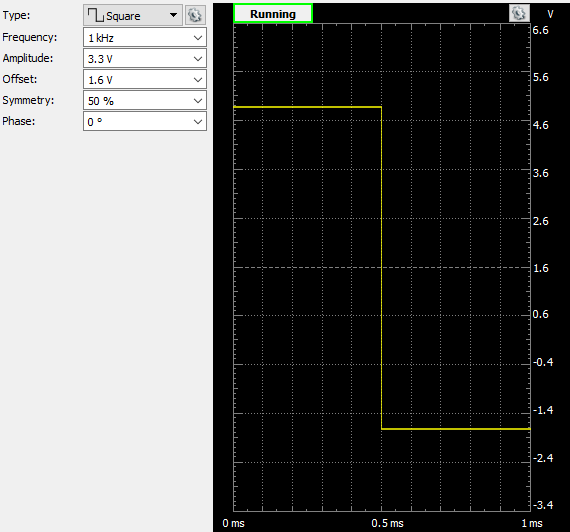
\includegraphics[width=0.3\textwidth]{Images/Implementation/Motor_controller_frequency}
		\label{fig:motor_controller_frequency}
	}
	\hfill
	\subfloat[Measurement setup, left: oscilliscope, right power and frequency generator]{
		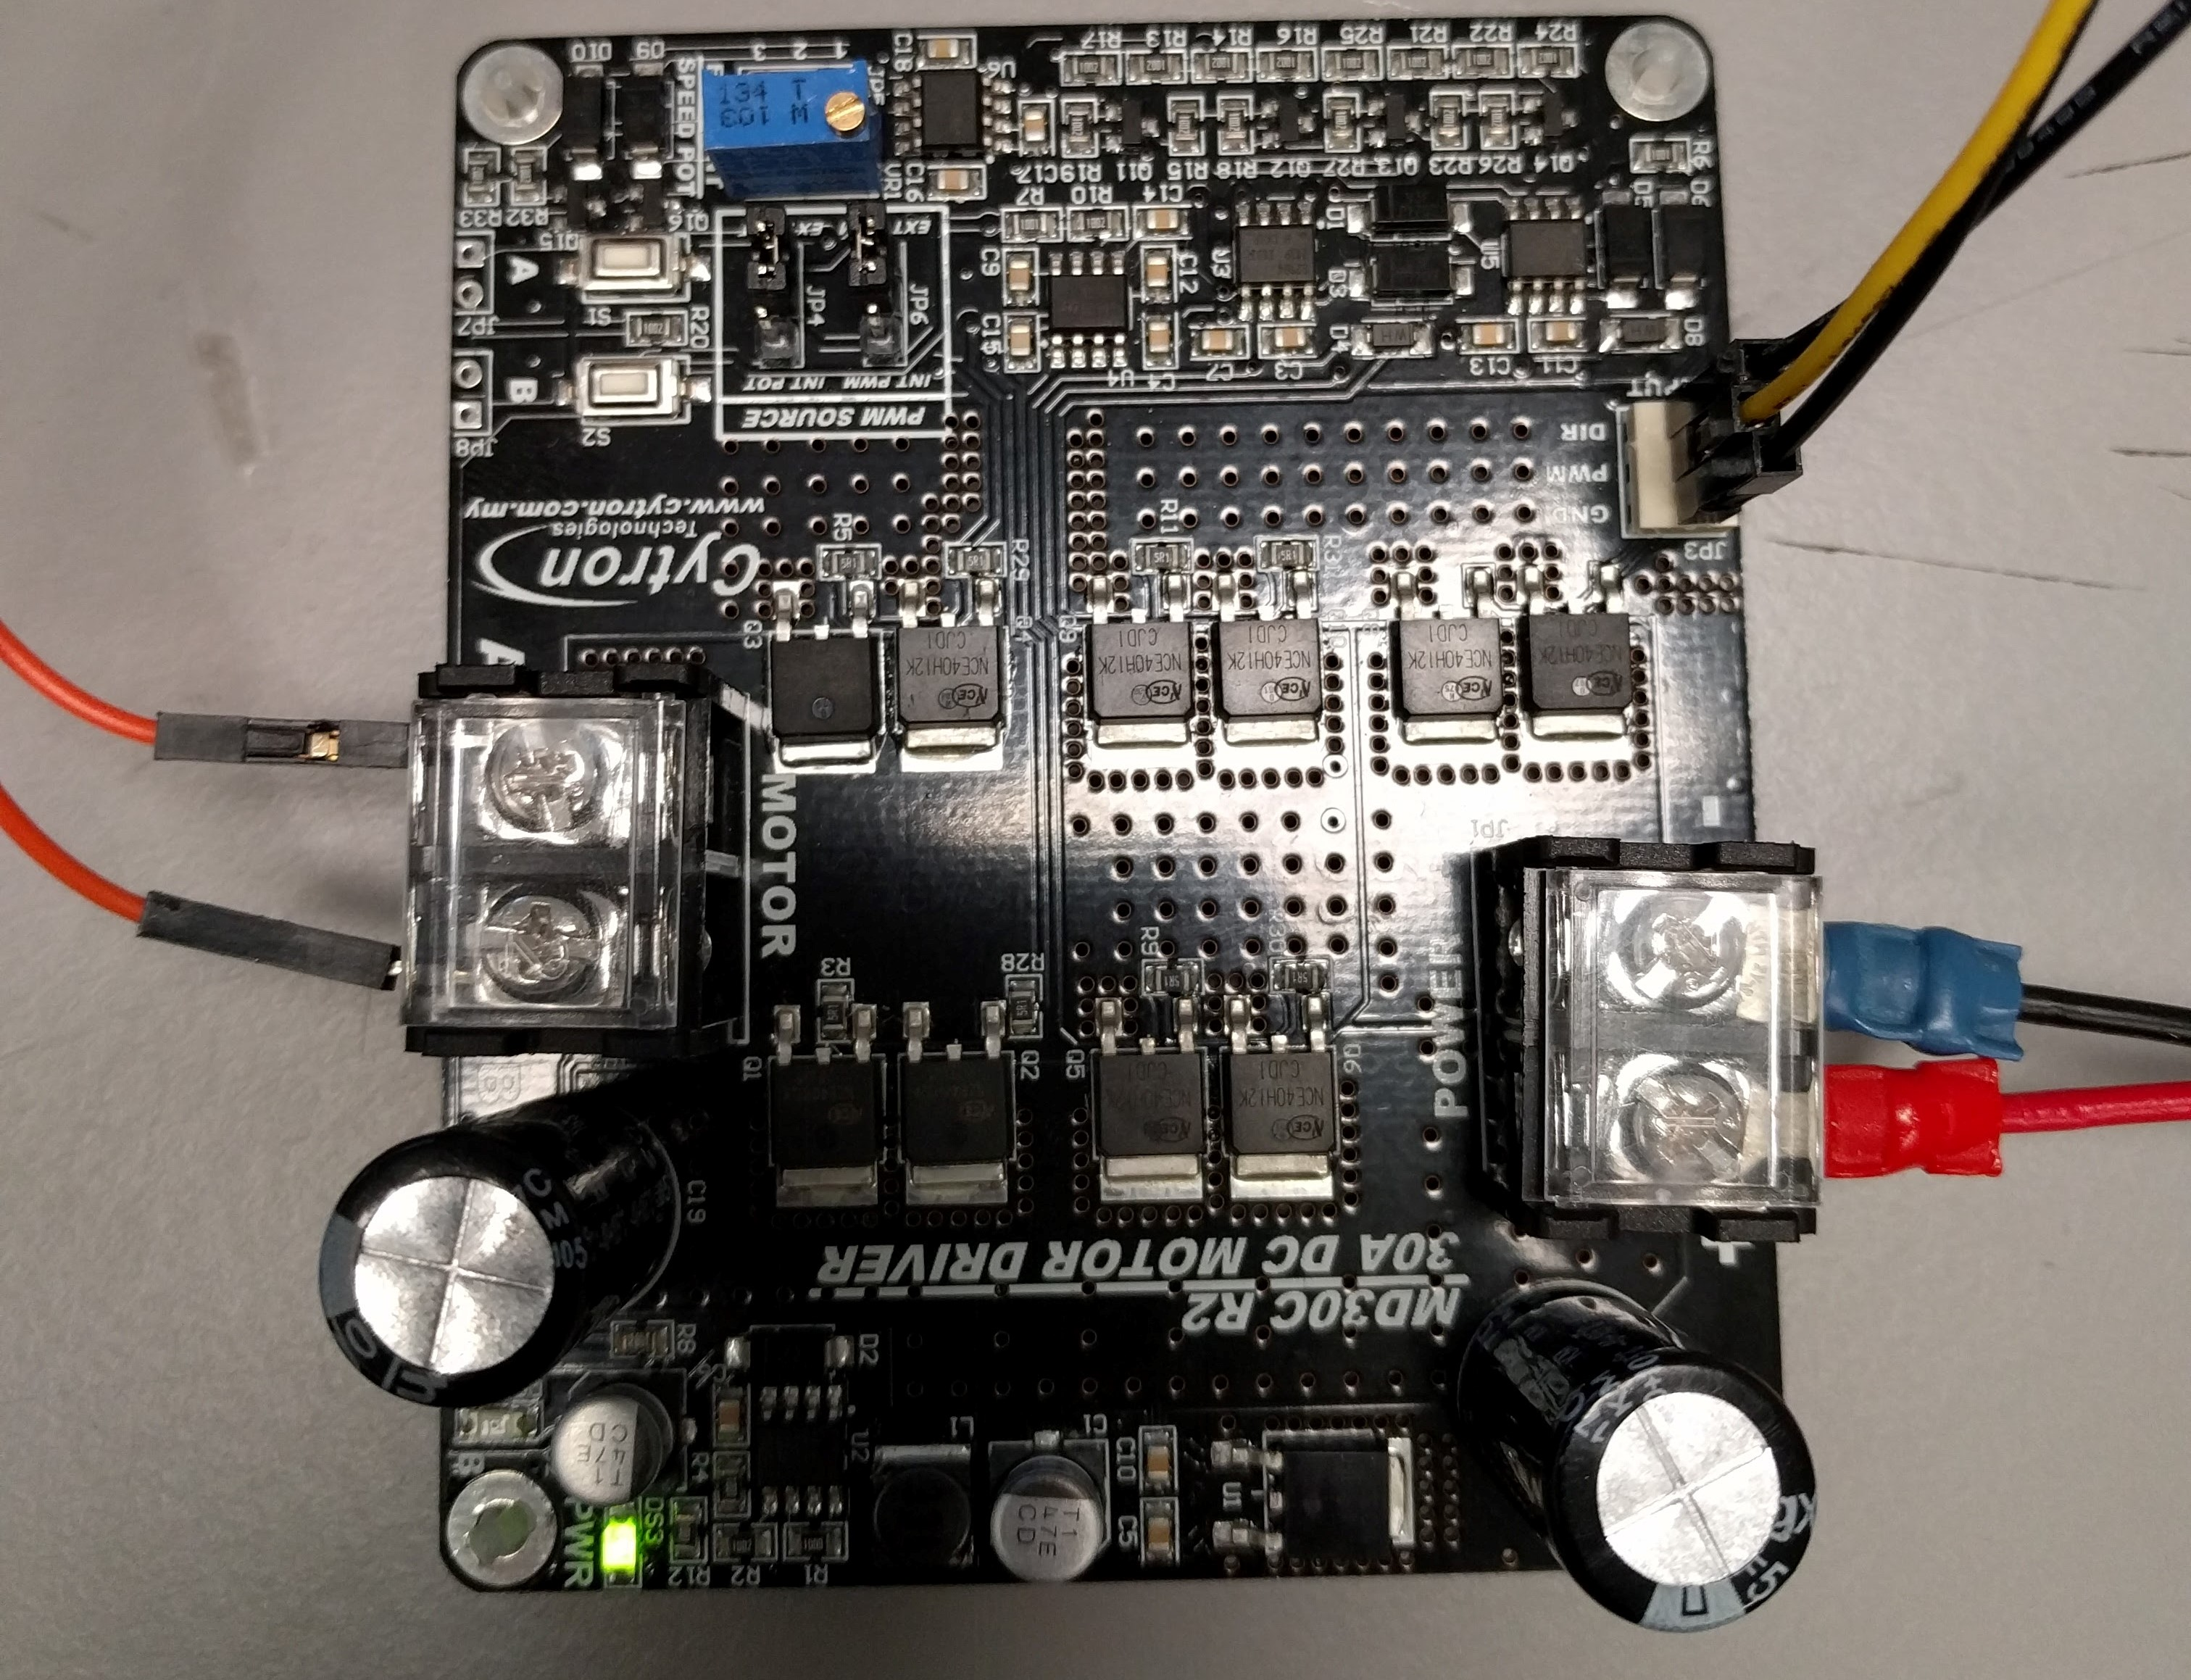
\includegraphics[width=0.3\textwidth]{Images/Implementation/Motor_controller_setup}
		\label{fig:motor_controller_setup}
	}
	\hfill
	\subfloat[Ouput on oscilloscope, 11~V peak to peak, 30~kHz square wave, 38~\% dutycycle]{
		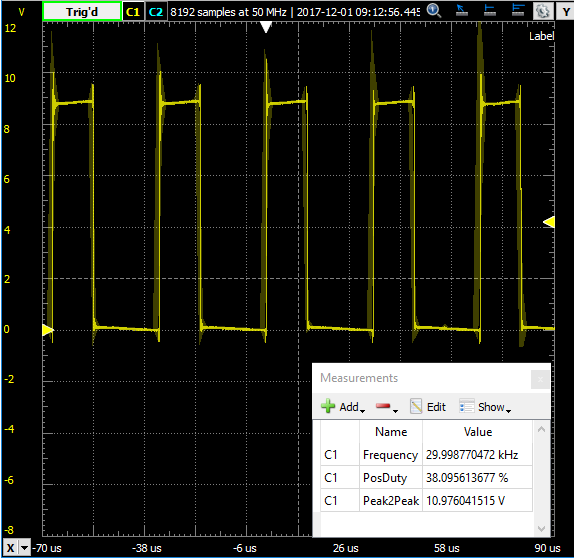
\includegraphics[width=0.3\textwidth]{Images/Implementation/Motor_controller_measurement}
		\label{fig:motor_controller_measurement}
	}
	\caption{Motor controller test}
\end{figure}

Another important consideration with the motor controller is how much current it draws on the input PWM signal. This is important because the Raspberry Pi which is going to drive the motor controller PWM input. It is widely assumed to only deliver up to 50 mA \cite{rpi-current}. which means that the motor controller should require less then that.

So to test the current draw, a multimeter is put in-line with the PWM signal from the frequency generator. The multimeter is set to measure amperes. This test results in a current draw of 0.21 mA as seen on figure~\ref{fig:pwmcurrentdraw}, which is easily with in the specification for the Raspberry Pi.

\begin{figure}[H]
\centering
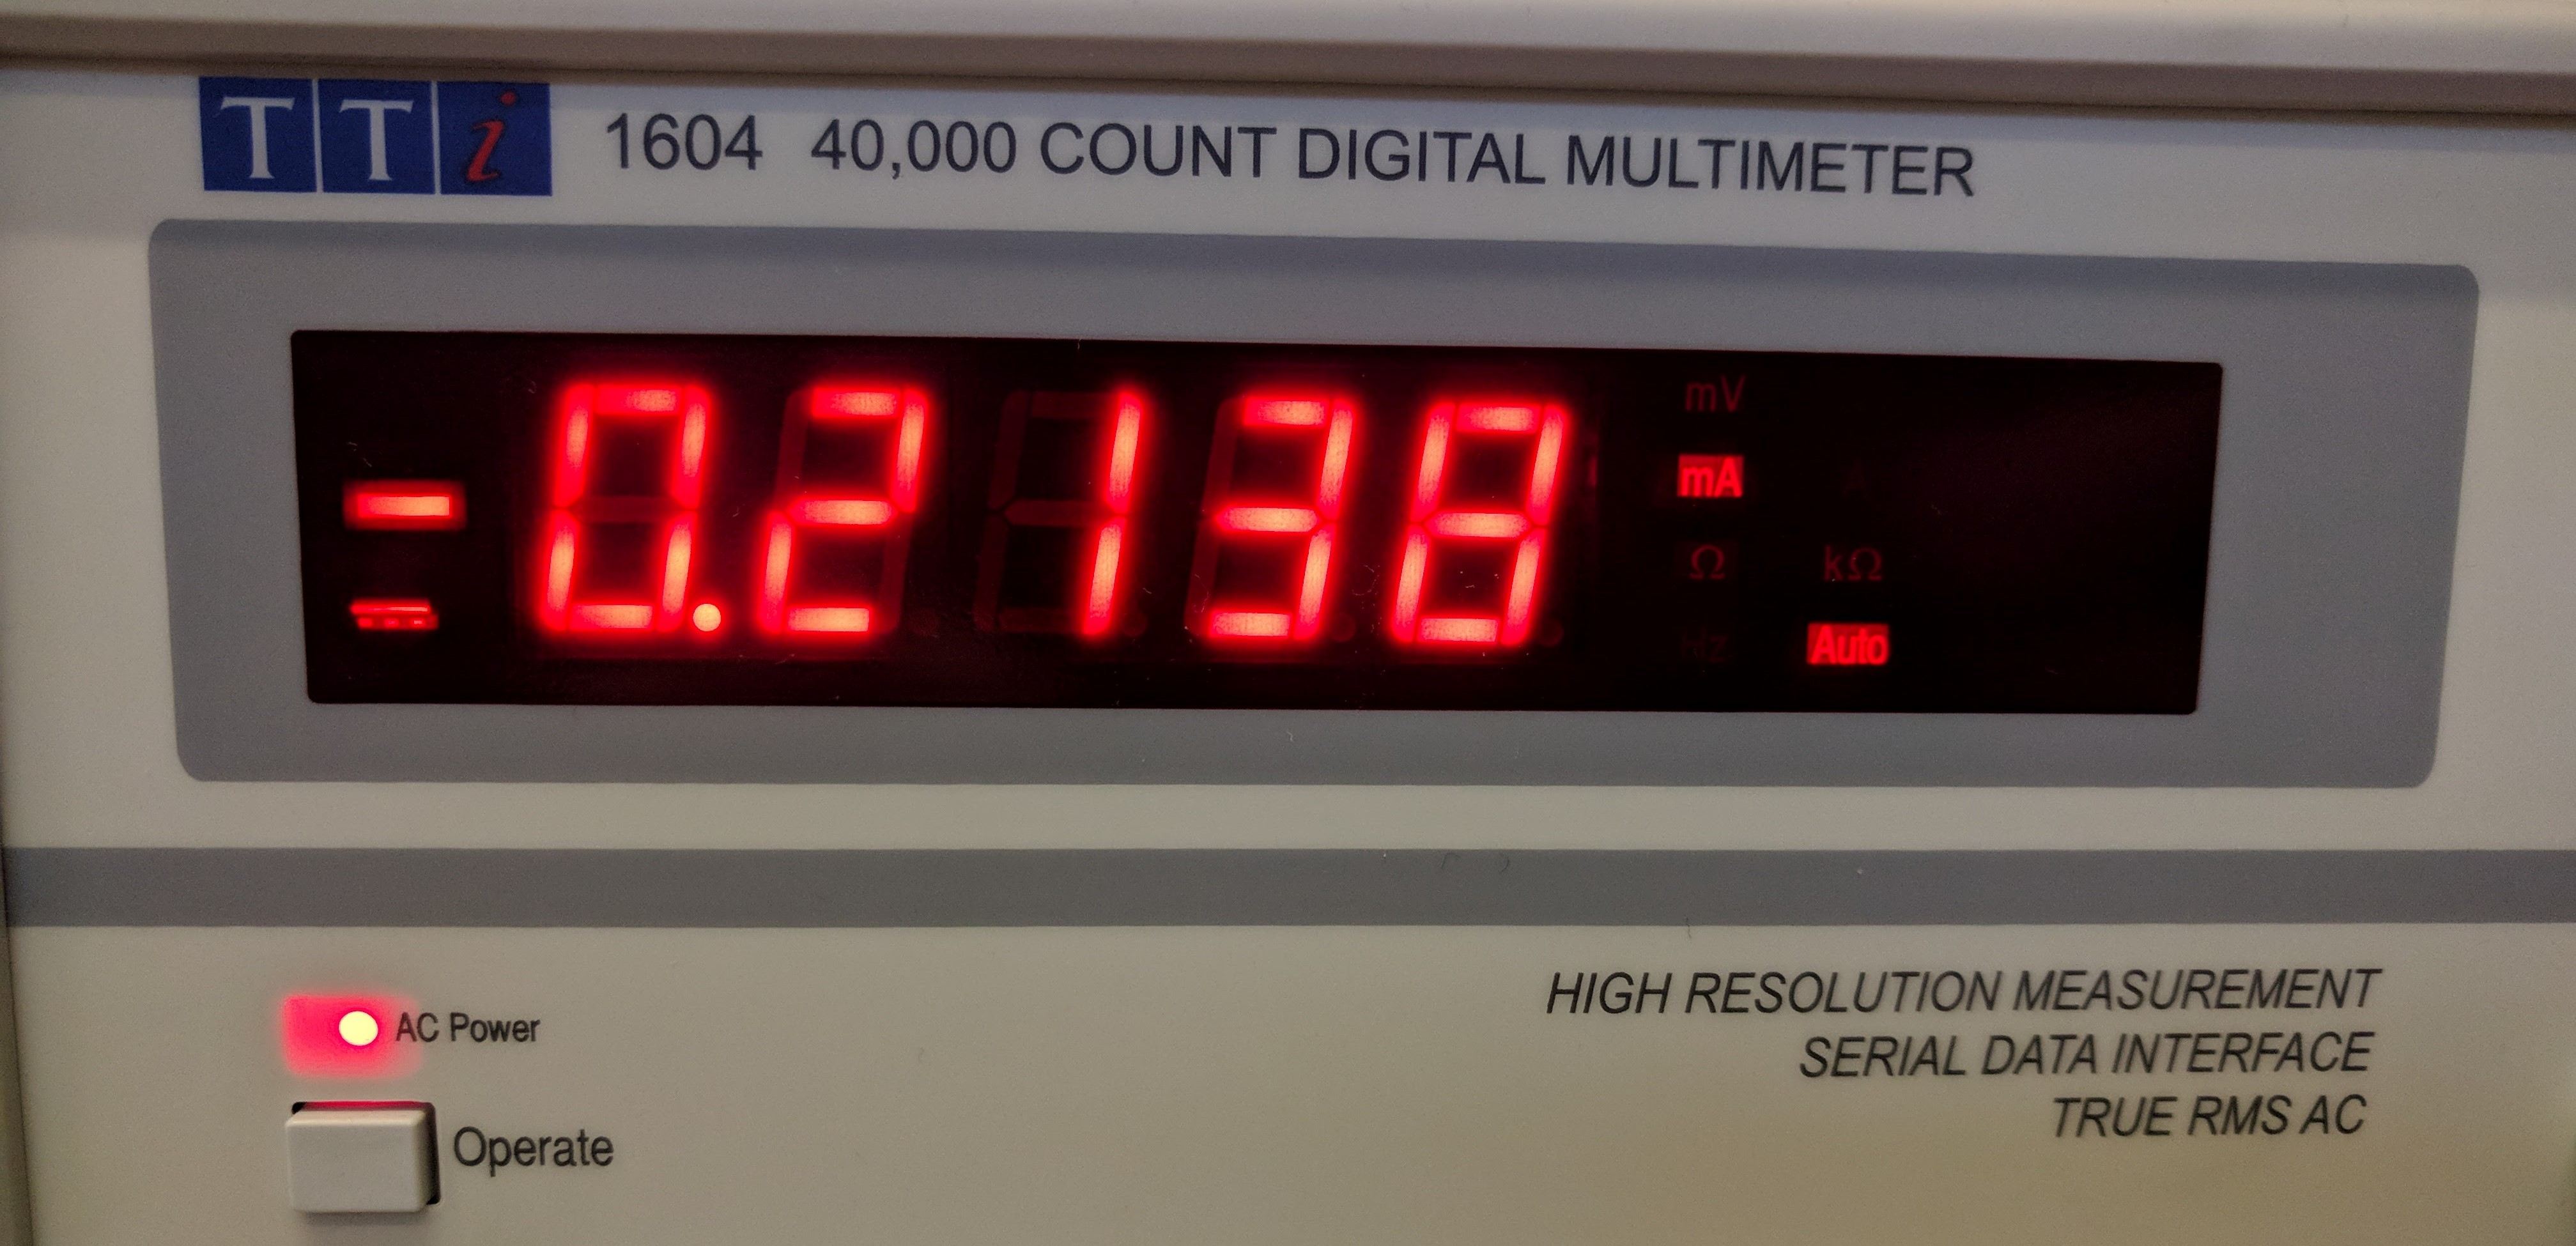
\includegraphics[width=0.4\linewidth]{Images/Implementation/pwm_current_draw}
\caption{Current draw on the PWM pin}
\label{fig:pwmcurrentdraw}
\end{figure}

\subsection{GPS}
The chosen GPS receiver, the neo-7m-0-000, comes with a windows software packages, which enables testing of the GPS receiver with out needing to write any code yourself. It is called u-center, it allows for GPS telegram output as well as a bunch of handy displays. It can display the amount of satellites, the fix status, and map of where the GPS receiver is located at. 

\begin{figure}[H]
\centering
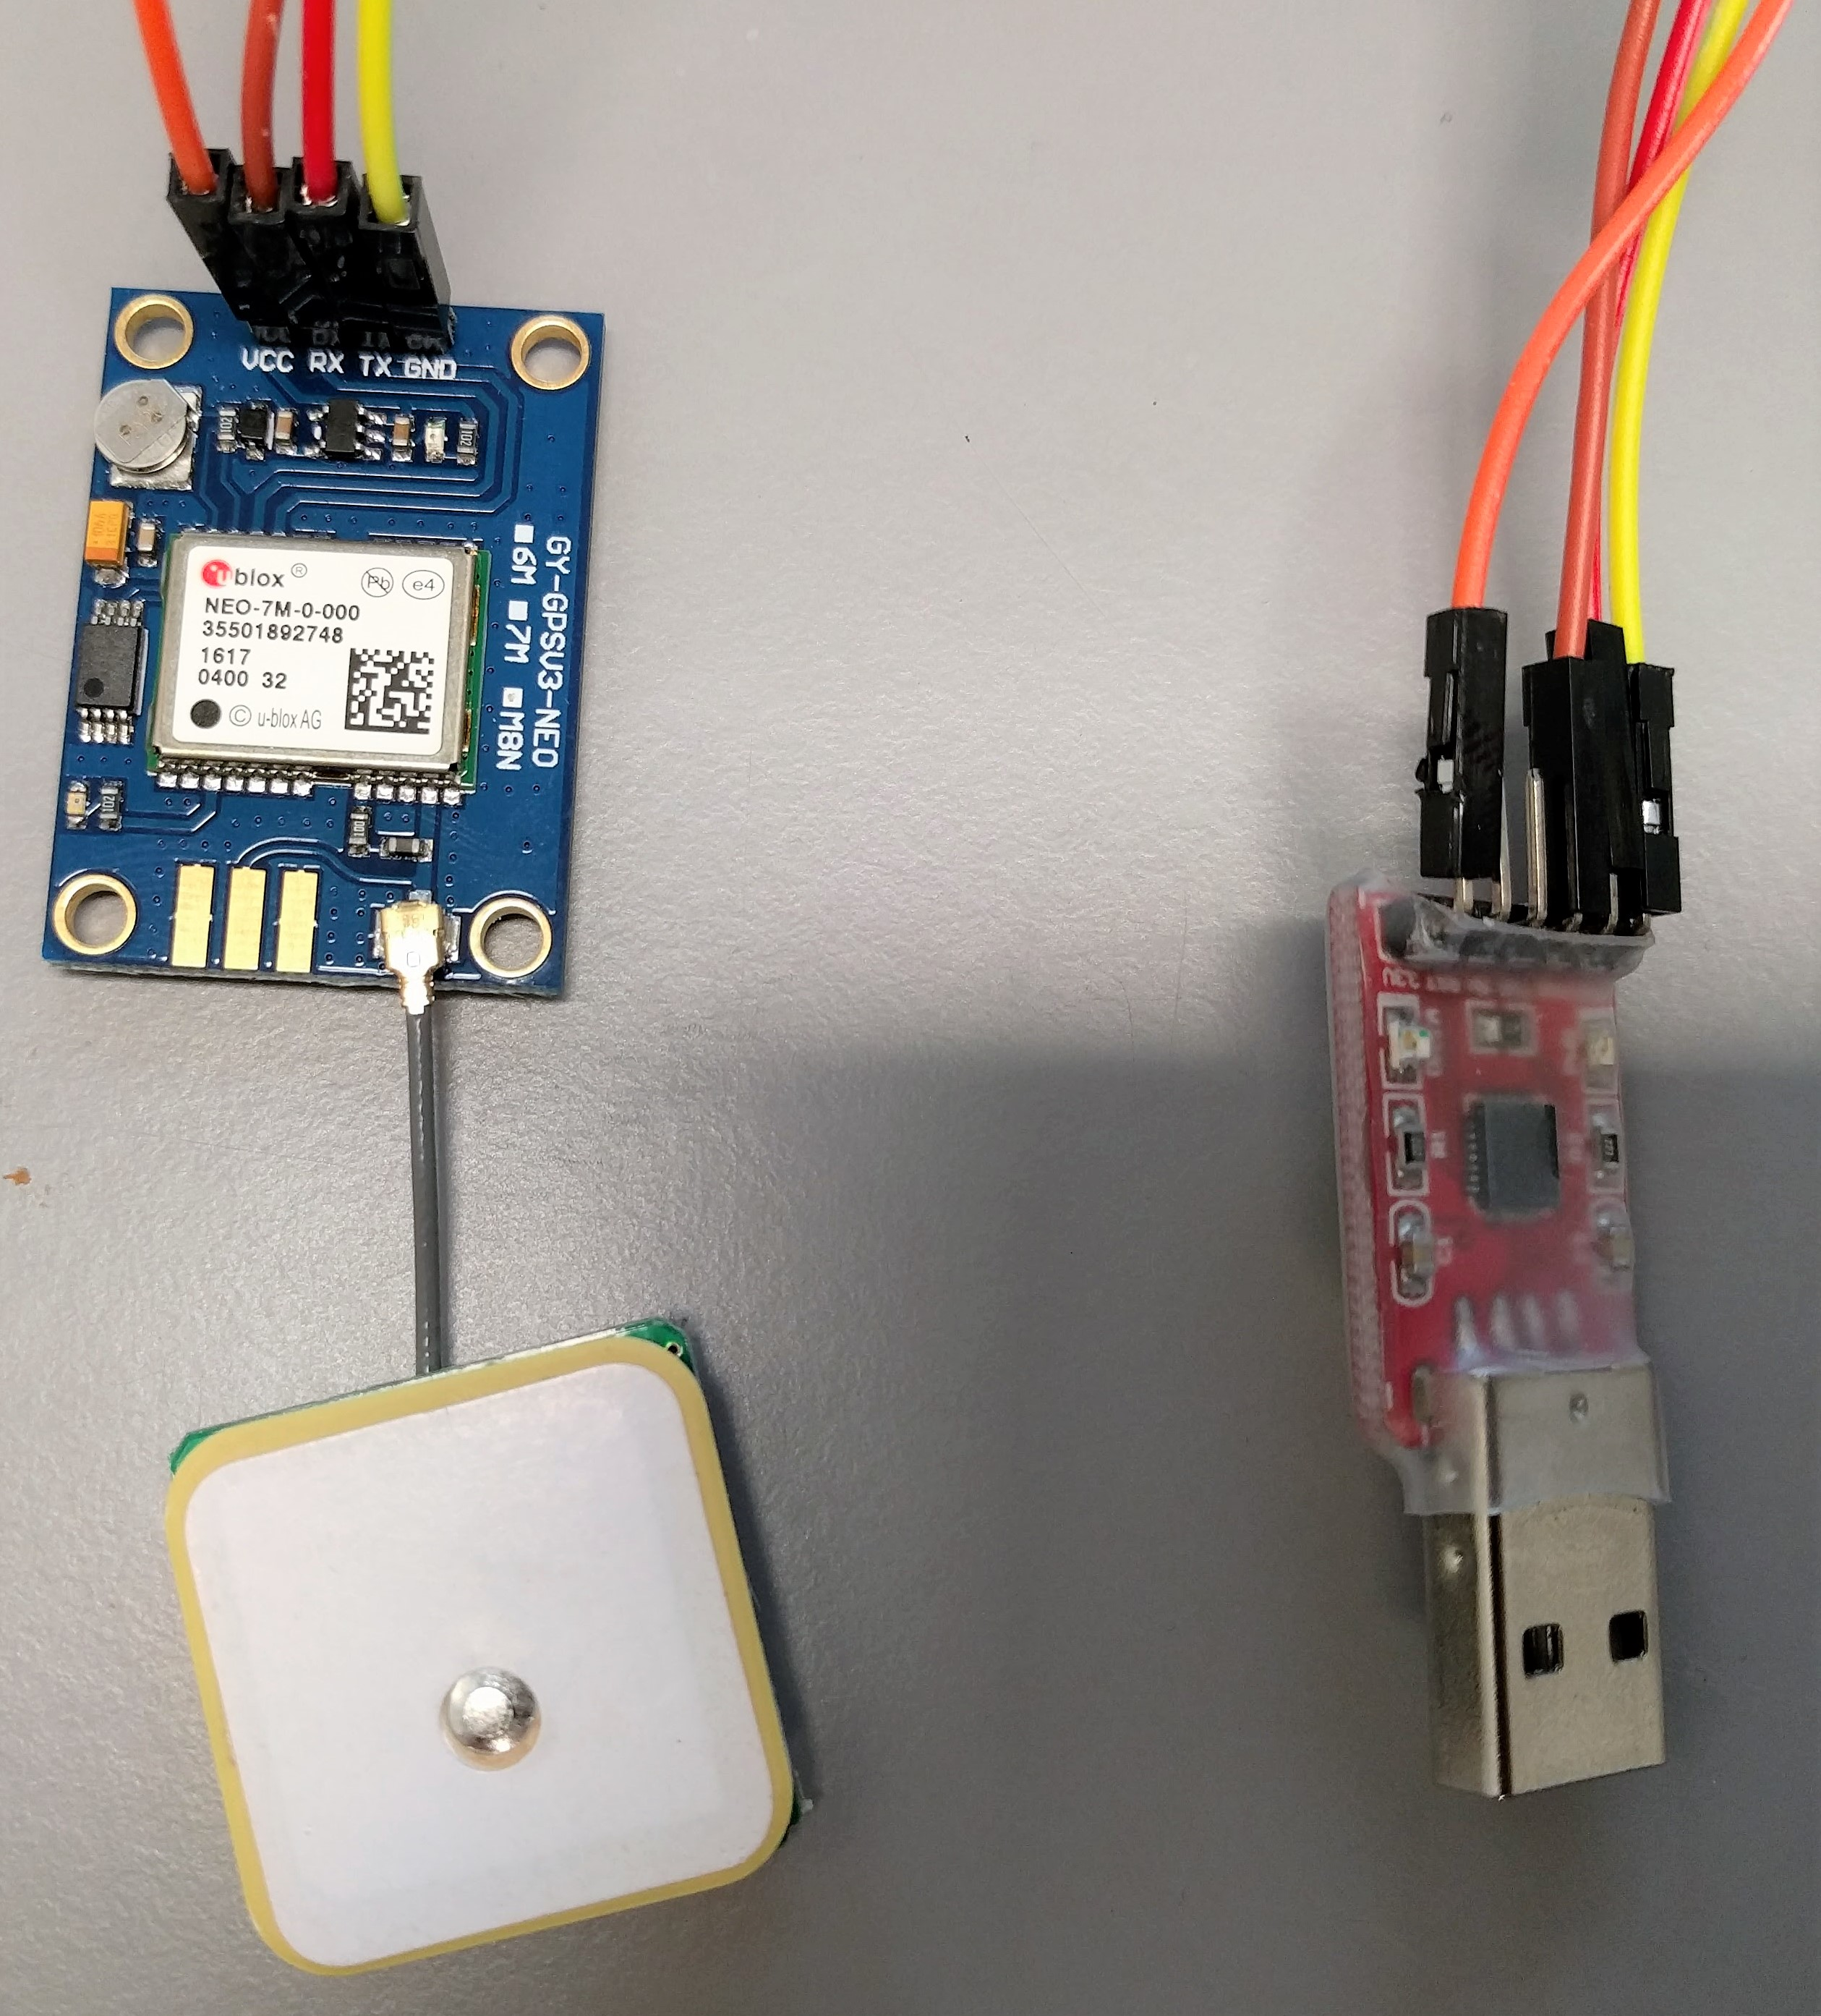
\includegraphics[width=0.4\linewidth]{Images/Implementation/gps_setup}
\caption{Gps setup with USB to serial converter}
\label{fig:gps_test_setup}
\end{figure}


To test and see if the GPS receiver is outputting something that can be used, and works. A test can be performed with u-center. First the GPS needs to be connected to a PC with USB to serial converter as show on figure~\ref{fig:gps_test_setup}. Then it needs to be connected in u-center, after this the receiver needs to be somewhere it can see the satellites, usually outside. After a cold start of around 30 seconds, it gets a fix, meaning it knows where it is. On figure~\ref{fig:gps_ucenter} a fix has been acquired and the receiver is outputting NMEA telegrams. a sample of these can be seen in listing~\ref{lst:gps_ucenter}

\begin{figure}[H]
\centering
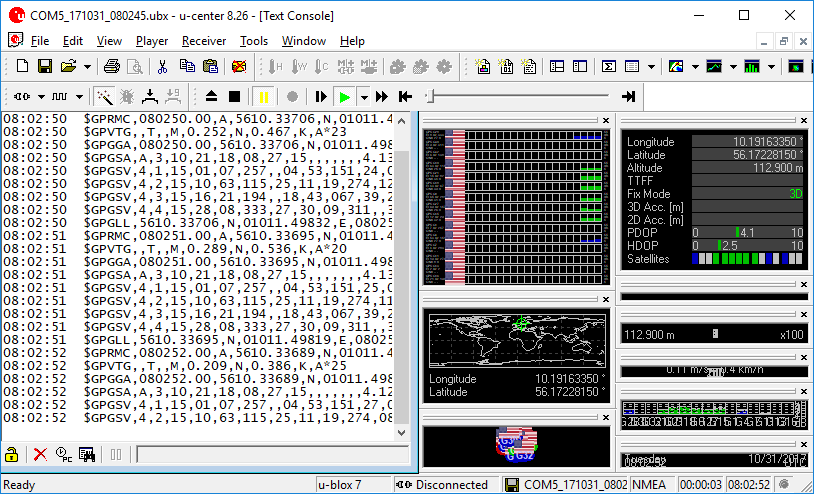
\includegraphics[width=1\linewidth]{Images/Implementation/ucenter_gps_test}
\caption{U-center software, where the GPS receiver has gotten a fix}
\label{fig:gps_ucenter}
\end{figure}

\begin{lstlisting}[caption = {Sample output of NMEA telegram when GPS receiver has fix in u-center. Timestamp removed}, captionpos=b, label={lst:gps_ucenter},firstnumber=1]
$GPGGA,080250.00,5610.33706,N,01011.49832,E,1,06,2.51,70.9,M,42.8,M,,*65
$GPGSA,A,3,10,21,18,08,27,15,,,,,,,4.13,2.51,3.28*09
$GPGSV,4,1,15,01,07,257,,04,53,151,24,07,04,283,,08,65,281,31*77
$GPGSV,4,2,15,10,63,115,25,11,19,274,12,13,02,002,,15,12,029,33*79
$GPGSV,4,3,15,16,21,194,,18,43,067,39,21,15,082,34,27,69,157,28*7E
$GPGSV,4,4,15,28,08,333,27,30,09,311,,32,06,138,*4D
$GPGLL,5610.33706,N,01011.49832,E,080250.00,A,A*60
$GPRMC,080251.00,A,5610.33695,N,01011.49819,E,0.289,,311017,,,A*7C
$GPVTG,,T,,M,0.289,N,0.536,K,A*20
\end{lstlisting}

\subsection{Raspberry Pi}
The Raspberry Pi should be able to drive the motor with a 30kHz PWM, and the servo with a 50 Hz PWM.
So to figure out if it is capable of this, two small test scripts can be written. To start with lets have a look at the servo.
\begin{lstlisting}[caption = {Test code to make the Raspberry pi run a servo}, captionpos=b, label={lst:rpi_servo}, language=C++,firstnumber=1]
#include <pigpio.h>

int main (){
        gpioInitialise();

        gpioSetMode(18,1); //Pin 18 pwm0 to output
        while(1){
                gpioServo(18,1500);
        }
}
\end{lstlisting}

To get the Raspberry Pi to output to its GPIO pins a library can be used. This library is the same that is going to be used for the software, and it's called pigpio \cite{pigpio}, as it can be seen in listing~\ref{lst:rpi_servo}. It has a function called \texttt{gpioServo}, which takes a value between 500 and 2500, which is the period lengths in microseconds. It automatically sets the frequency to 50 Hz. Also the GPIO need to be initialized with \texttt{gpioInitialise}, and the output mode needs to be set to 1 meaning output, with \texttt{gpioSetMode}. The output pin is set to 18. 

\begin{figure}[H]
\centering
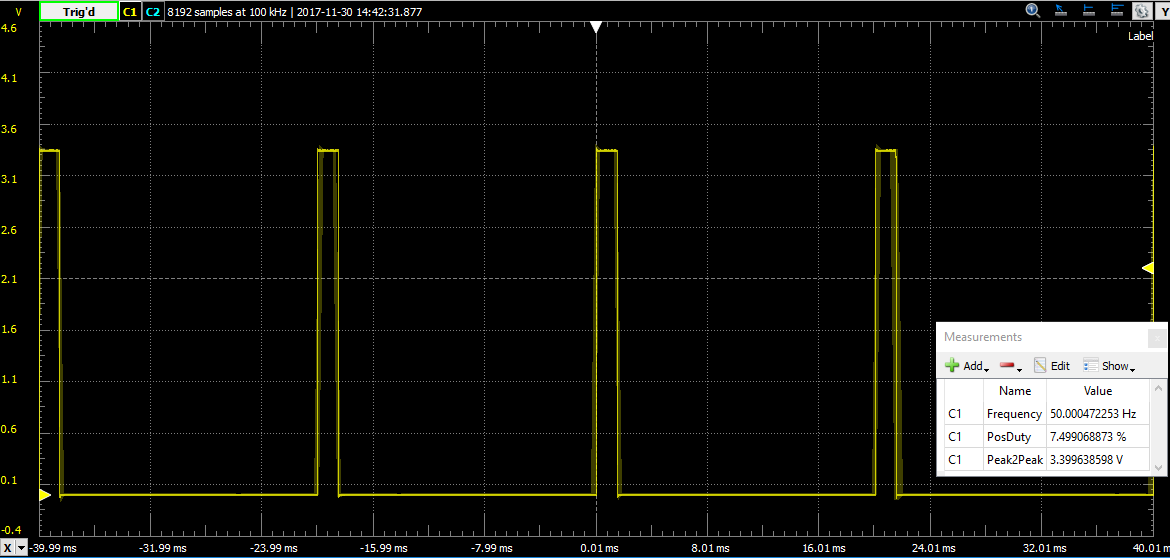
\includegraphics[width=0.7\linewidth]{Images/Implementation/RPI_servo_PWM}
\caption{Oscilloscope measurement of pin 18 on Raspberry pi, with servo test code}
\label{fig:rpi_servo_pwm}
\end{figure}

Now that the servo signal is set up it can be measured with an oscilloscope. In figure~\ref{fig:rpi_servo_pwm}, on the oscilloscope there is a signal with a frequency of 50 Hz, and a duty cycle of 7.5 \% which translates to a period time of 1.5 ms, which is the same as was setup in the test code.

The exact same thing can be done to test whether or not Raspberry Pi is able to output a 30 kHz signal, this time a new piece of test code is need, it can be seen in listing~\ref{lst:rpi_motor}. Just like before the GPIO library need to be initialized, and the pin needs to be set to be an output. This time the function \texttt{gpioHardwarePWM} is used to be able to set a high PWM frequency, and a duty cycle with a high degree of steps. The frequency is set to 30.000 Hz or 30 kHz and the duty cycle is set to 10.000 which is equivalent to 1\% since the highest duty cycle is 1.000.000. The output pin is like before pin 18.

\begin{lstlisting}[caption = {Test code to make the Raspberry pi run a motor a 30kHz}, captionpos=b, label={lst:rpi_motor}, 
language=C++,firstnumber=1]
#include <pigpio.h>

int main (){
        gpioInitialise();

        gpioSetMode(18,1); //Pin 18 pwm0 to output
        while(1){
                gpioHardwarePWM(18,30000,10000);
        }
}
\end{lstlisting}

Just like be with the servo the oscilloscope output can be seen on figure~\ref{fig:rpi_motor_pwm}. The frequency measured is 30 kHz and the duty cycle is just about 1\%. This means that the Raspberry Pi is capable of driving the motor driver with a frequency high enough to avoid a whining sound, as discussed in section~\ref{sec:motor_controller}: \nameref{sec:motor_controller}.

\begin{figure}[H]
\centering
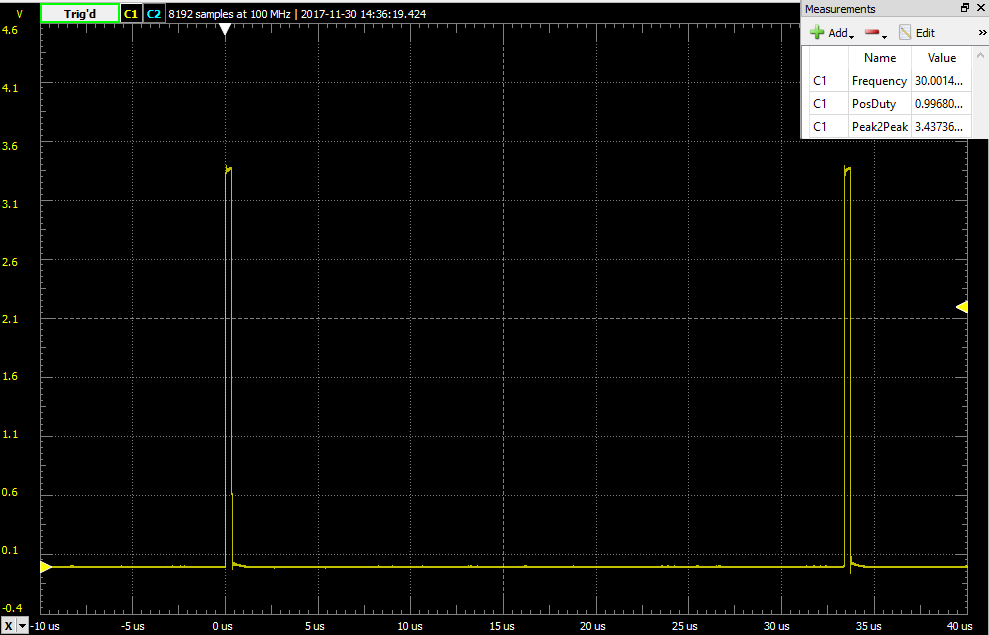
\includegraphics[width=0.7\linewidth]{Images/Implementation/RPI_motor_PWM}
\caption{Oscilloscope measurement of pin 18 on Raspberry pi, with motor test code}
\label{fig:rpi_motor_pwm}
\end{figure}


Now the last thing that the Raspberry Pi needs is to interface with the GPS receiver. Which is easily accomplished with the built in GPIO serial interface that the Raspberry Pi comes with. But before it can be used, the serial console has to be disabled. This console is used to communicate with the Raspberry pi headlessly, meaning that a PC can connect to it with a serial interface. The serial console is disable with \texttt{raspbi-config}, it is important not to disable the serial hardware along with the console. Once this is done, a serial interface called \texttt{/dev/ttyS0} is enabled. With the software library SimpleSerial\cite{simple_serial} it is easy to read the output of a GPS receiver since it ends all telegrams with a newline. A test program can be seen in listing~\ref{lst:gps_test}, and the resulting output can be seen in listing~\ref{lst:gps_test_output}. 


\begin{lstlisting}[caption = {Test code to make the Raspberry Pi output GPS receiver telegrams}, captionpos=b, label={lst:gps_test}, 
language=C++,firstnumber=1]
#include <iostream>
#include "CAPTAIN/SimpleSerial.h"

int main(){

        SimpleSerial serial("/dev/ttyS0",9600);

        while(1){
                std::cout << serial.ReadLine() << std::endl;
        }
}

\end{lstlisting}

\begin{lstlisting}[caption = {Output of the GPS receiver test code}, captionpos=b, label={lst:gps_test_output}, 
language=C++,firstnumber=1]
$GPGGA,,,,,,0,00,99.99,,,,,,*48
$GPGSA,A,1,,,,,,,,,,,,,99.99,99.99,99.99*30
$GPGSV,1,1,02,02,,,25,19,,,23*77
$GPGLL,,,,,,V,N*64
$GPRMC,,V,,,,,,,,,,N*53
$GPVTG,,,,,,,,,N*30
\end{lstlisting}

It is important to realize that there is not real data in the telegrams in listing~\ref{lst:gps_test_output}, this is because the test was conducted indoors, and thus the GPS receiver cannot gain fix. Still this proves that the Raspberry pi is capable of reading data from the GPS receiver.


%Servo ouput, images + code bit
%Pwm Output, images + code bit

\subsection{Level converter}
A level converter is needed in the system because the servo needs an input PWM signal of 5~V, and the Raspberry Pi outputs a 3.3V PWM signal. A level converter is a simple device it requires a supply from the low voltages side, in this case 3.3 V. Then it needs a supply from the high voltage side, 5~V. and then it converts the logic level from one supply to the other. The setup can be seen on~\ref{fig:levelshifter_setup}.

\begin{figure}[H]
\centering
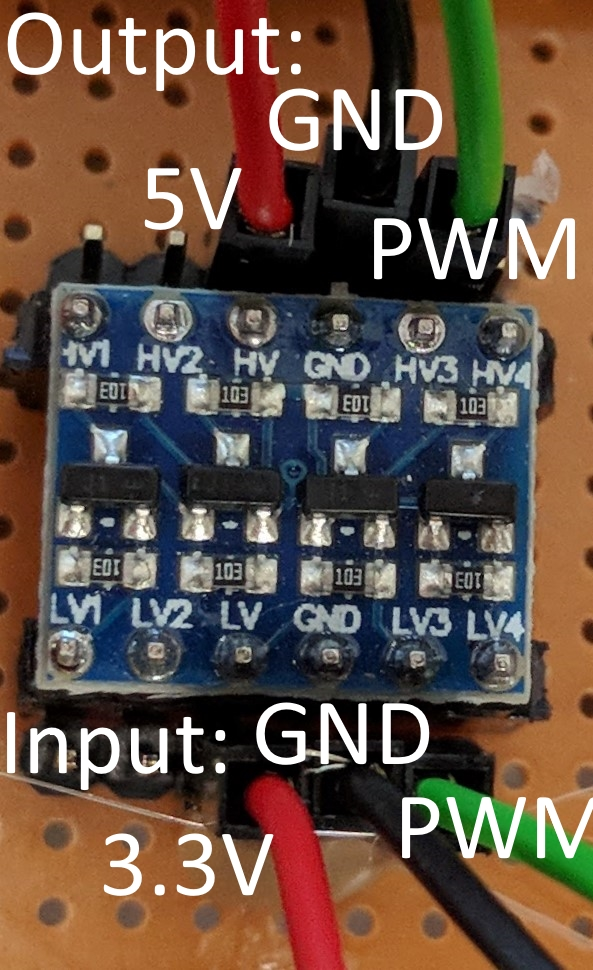
\includegraphics[width=0.3\linewidth]{Images/Implementation/level_shift_setup}
\caption{Level shifter setup}
\label{fig:levelshifter_setup}
\end{figure}

\subsection{Integration}
\label{sec:hardware_int}
Now that all the components have been tested they can be put together. For this purpose a perfboard\cite{perfboard} was put together, with the correct connectors and connection points.
To connect the battery to the perfboard and to connect perfboard to the motor, safety banana receptacles\cite{banana-connector} were used, like the one seen in figure~\ref{fig:banana_connector}. These were chosen since they are the highest amperage rated connectors in stock at the Department of Engineering. The banana receptacles are placed in two pairs, one for ground and one for the supply. The two pairs are connected with a thick gauge wire to accommodate the anticipated high current draw of the motor. 

\begin{figure}[h]
\centering
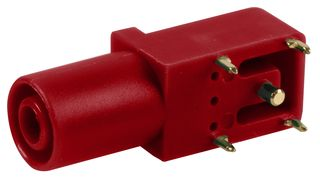
\includegraphics[width=0.3\linewidth]{Images/Design/safety-banana-receptical}
\caption{Safety banana receptacle\cite{banana-connector}}
\label{fig:banana_connector}
\end{figure}


On the perfboard male pin headers are used to distribute the battery voltage and ground. They are both connect to the two stepdown regulators, which in turn have two rows each of male pin headers to distribute the regulated voltage, as seen in figure~\ref{fig:integration}. 

\begin{figure}[h]
\centering
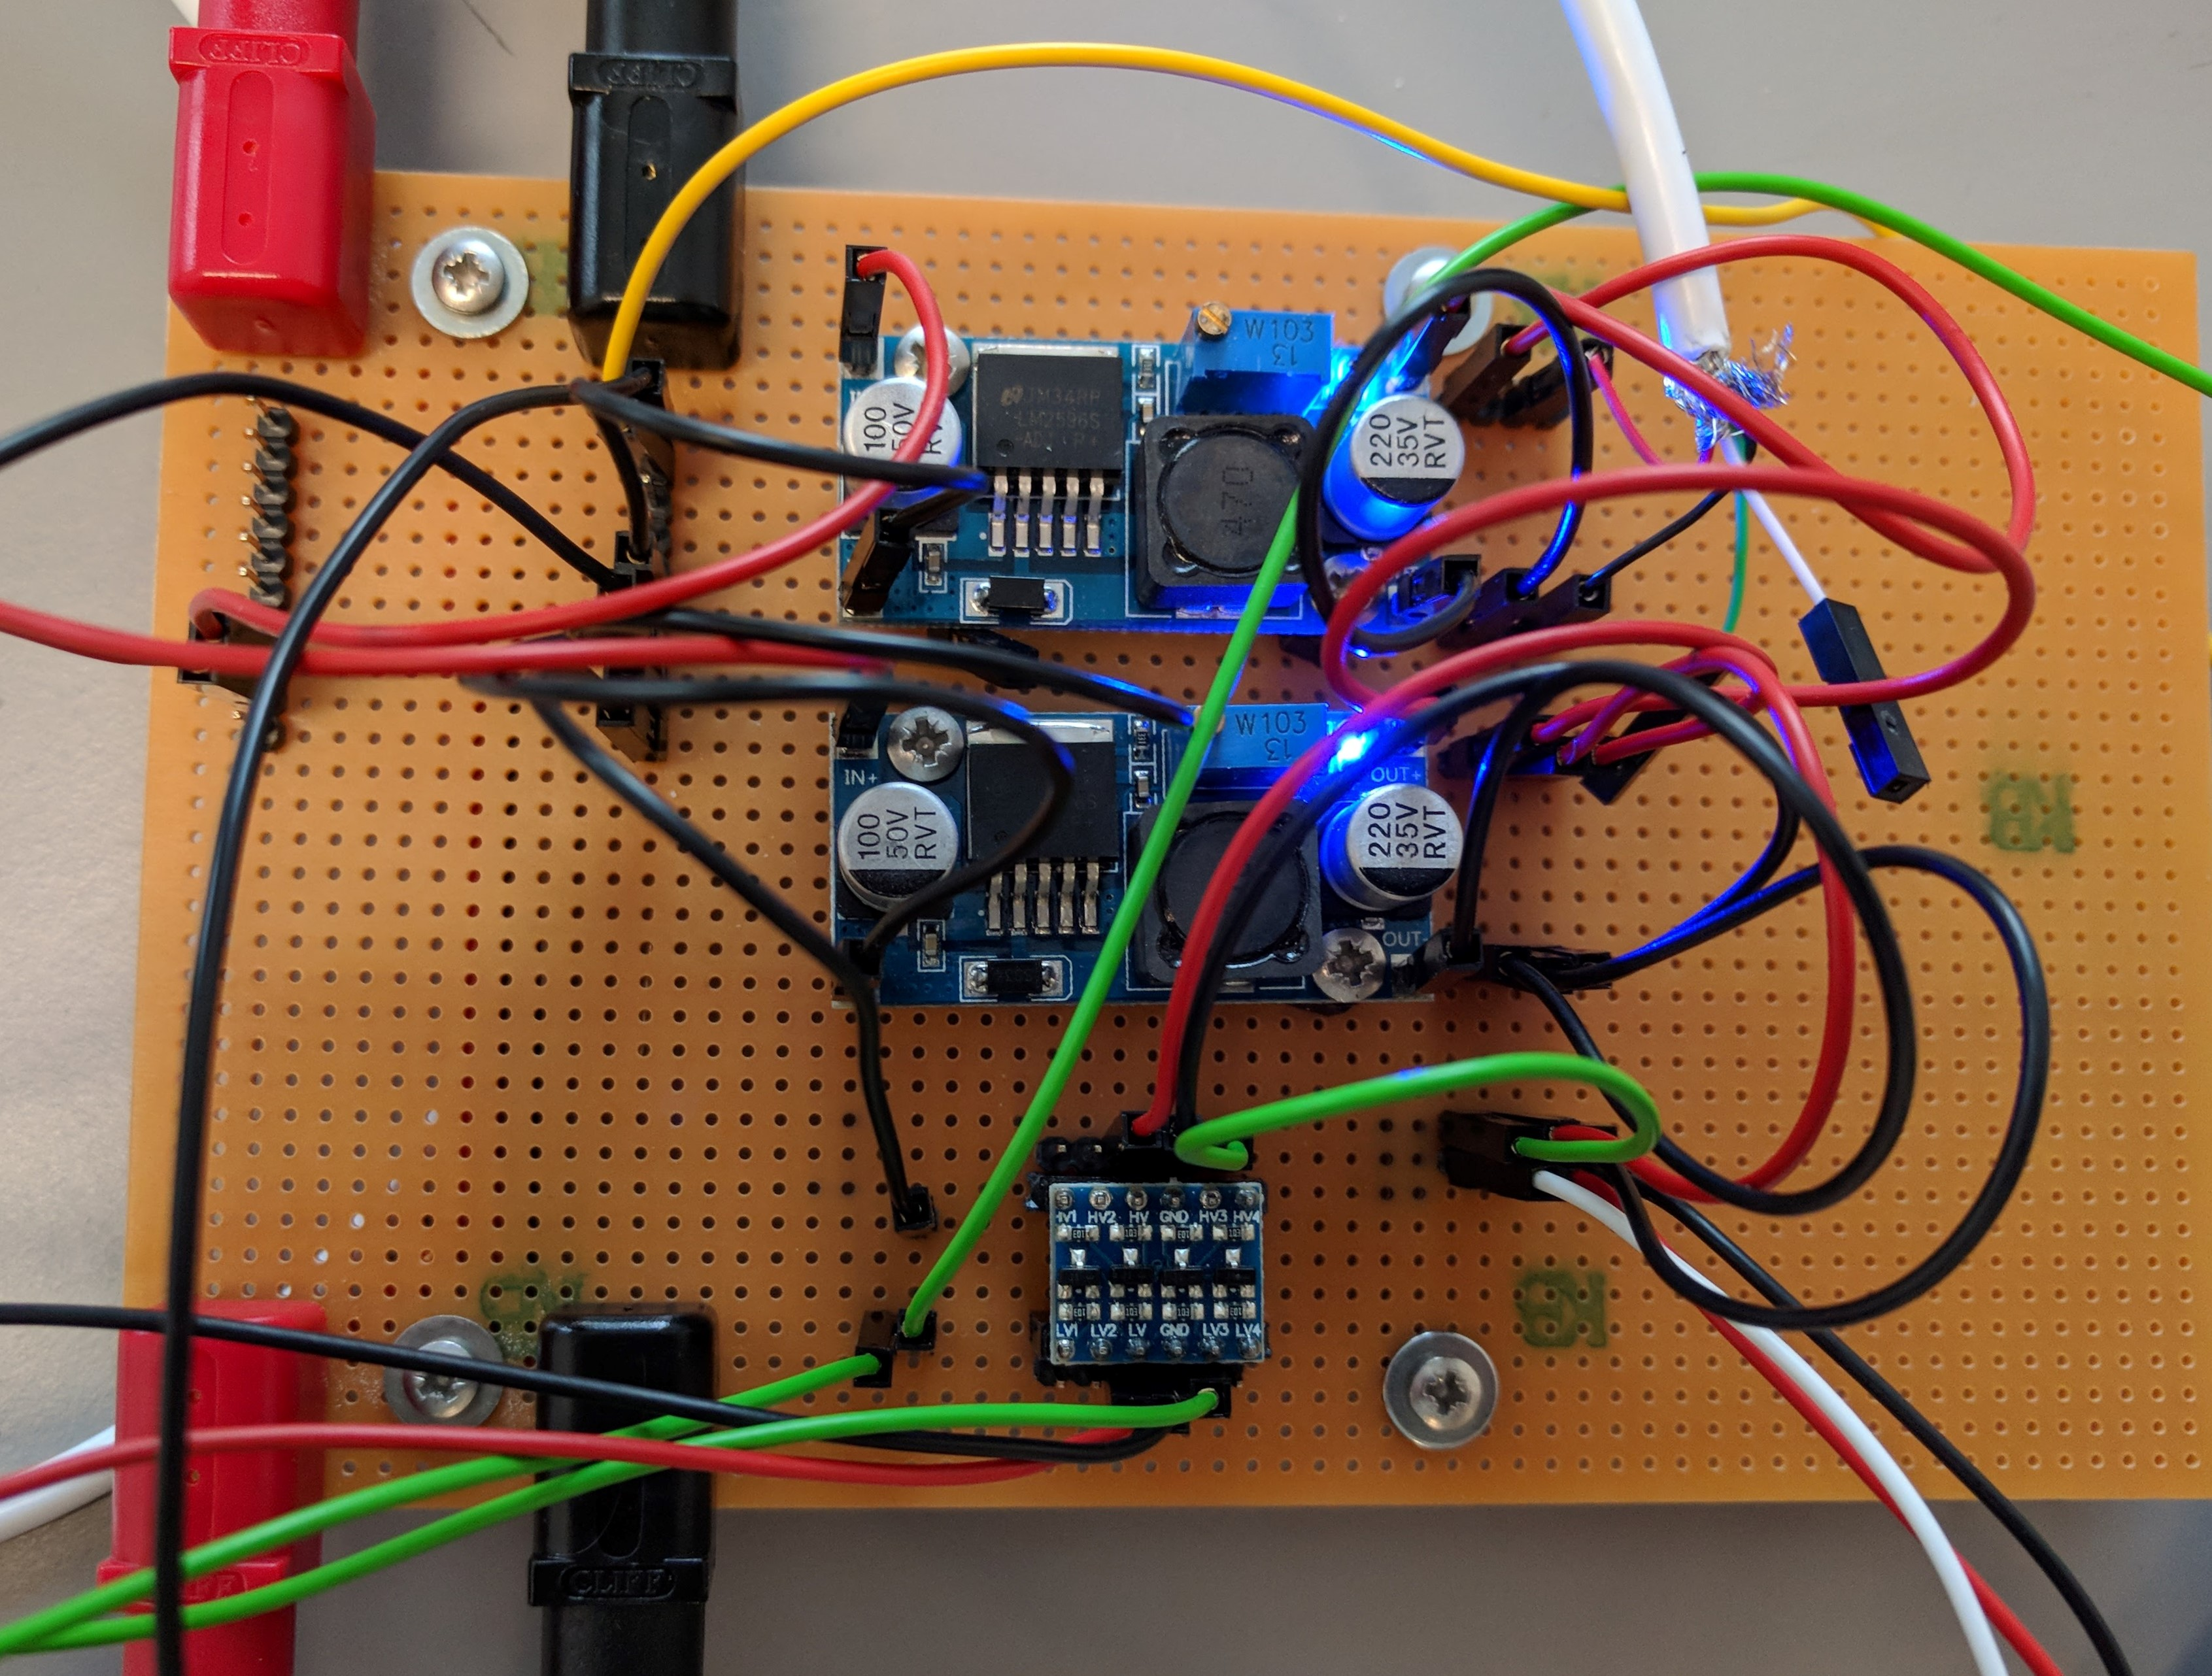
\includegraphics[width=0.7\linewidth]{Images/Implementation/integration}
\caption{All components on perfboard}
\label{fig:integration}
\end{figure}

All the components are connected with female to female pin header wires, which makes it easy to change the layout. This could be if component needs replacing or if the wiring it self needs to change.

The upper stepdown regulator in figure~\ref{fig:integration} is used to power the Raspberry Pi. The Raspberry Pi gets it power through a USB micro-b connector, which has been split into female pin headers. The pin headers are connected to the voltage regulator. 

To power the servo, the lower voltage regulator is used in figure~\ref{fig:integration}. The supply and ground are collected together with the 5~V PWM signal from the level converter, which is also powered from the 5~V supply of the lower regulator. The servo is connected to the collected wires. The 3.3~V PWM signal and 3.3~V supply comes from the Raspberry Pi and into the level converter.

The GPS receiver is directly connected and driven off of the Raspberry Pi's internal 3.3~V supply, the transmitter connection to GPS receiver pin was left unconnected, since it is never need, and can introduce some unwanted behavior if noise is induced on the wire.

The Motor need all the power it can gets, therefore the motor controller power is connected directly to the battery through the perfboard. The motor controller has a direction pin which is grounded on the perfboard, and the ground wire is also grounded, whilst the PWM wire is connected to the Raspberry Pi's hardware PWM pin. To insure that the motor doesn't turn on when the Raspberry Pi is not driving the PWM signal, a pull down resistor was added on to the perfboard. 

\begin{figure}[H]
\centering
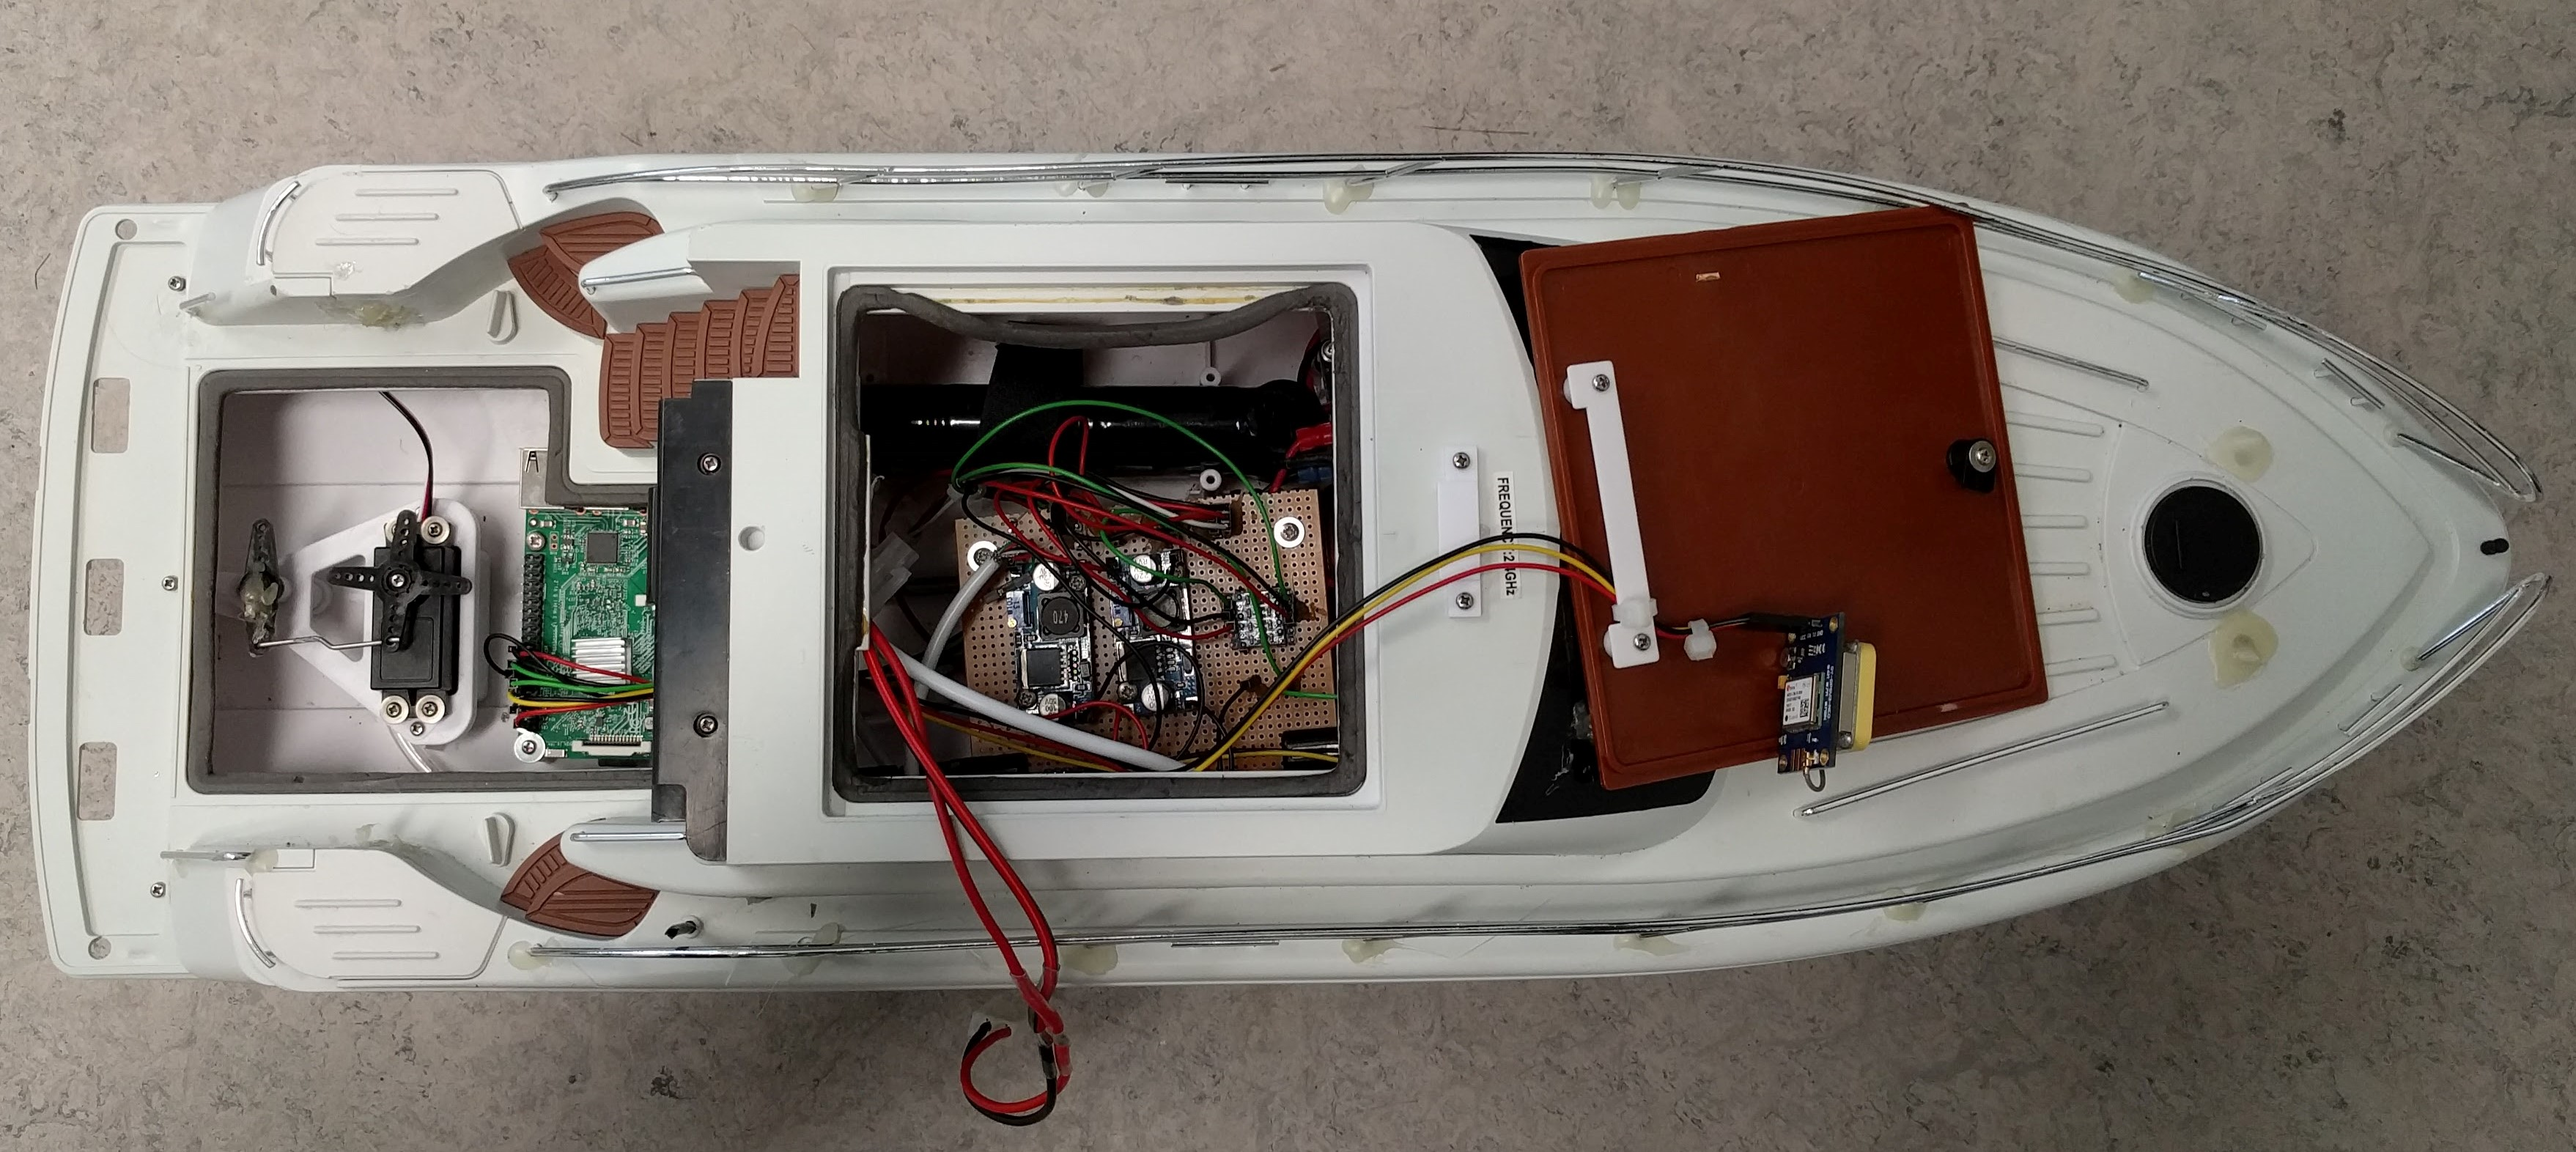
\includegraphics[width=0.7\linewidth]{Images/Implementation/all_hardware_in_boat}
\caption{Electronics hardware inside boat}
\label{fig:electronics_boat}
\end{figure}

The last thing that is required, is to enclose all of electronics hardware in side the boat. The motor position is fixed in side the boat and so is the servo, that means that the electronics need to sit around it. The Raspberry Pi is positioned in the stern of the boat together with the servo. The motor controller is in the bow of the boat. The perfboard is in the middle of the boat atop the motor. Lastly the GPS receiver is cable tied to the lid that is used to seal the boat, this is do to get the GPS receiver to the highest position. The positions described can be seen in figure~\ref{fig:electronics_boat}, and the closed boat with all the hardware inside can be seen in figure~\ref{fig:boat_closed}.

\begin{figure}[H]
\centering
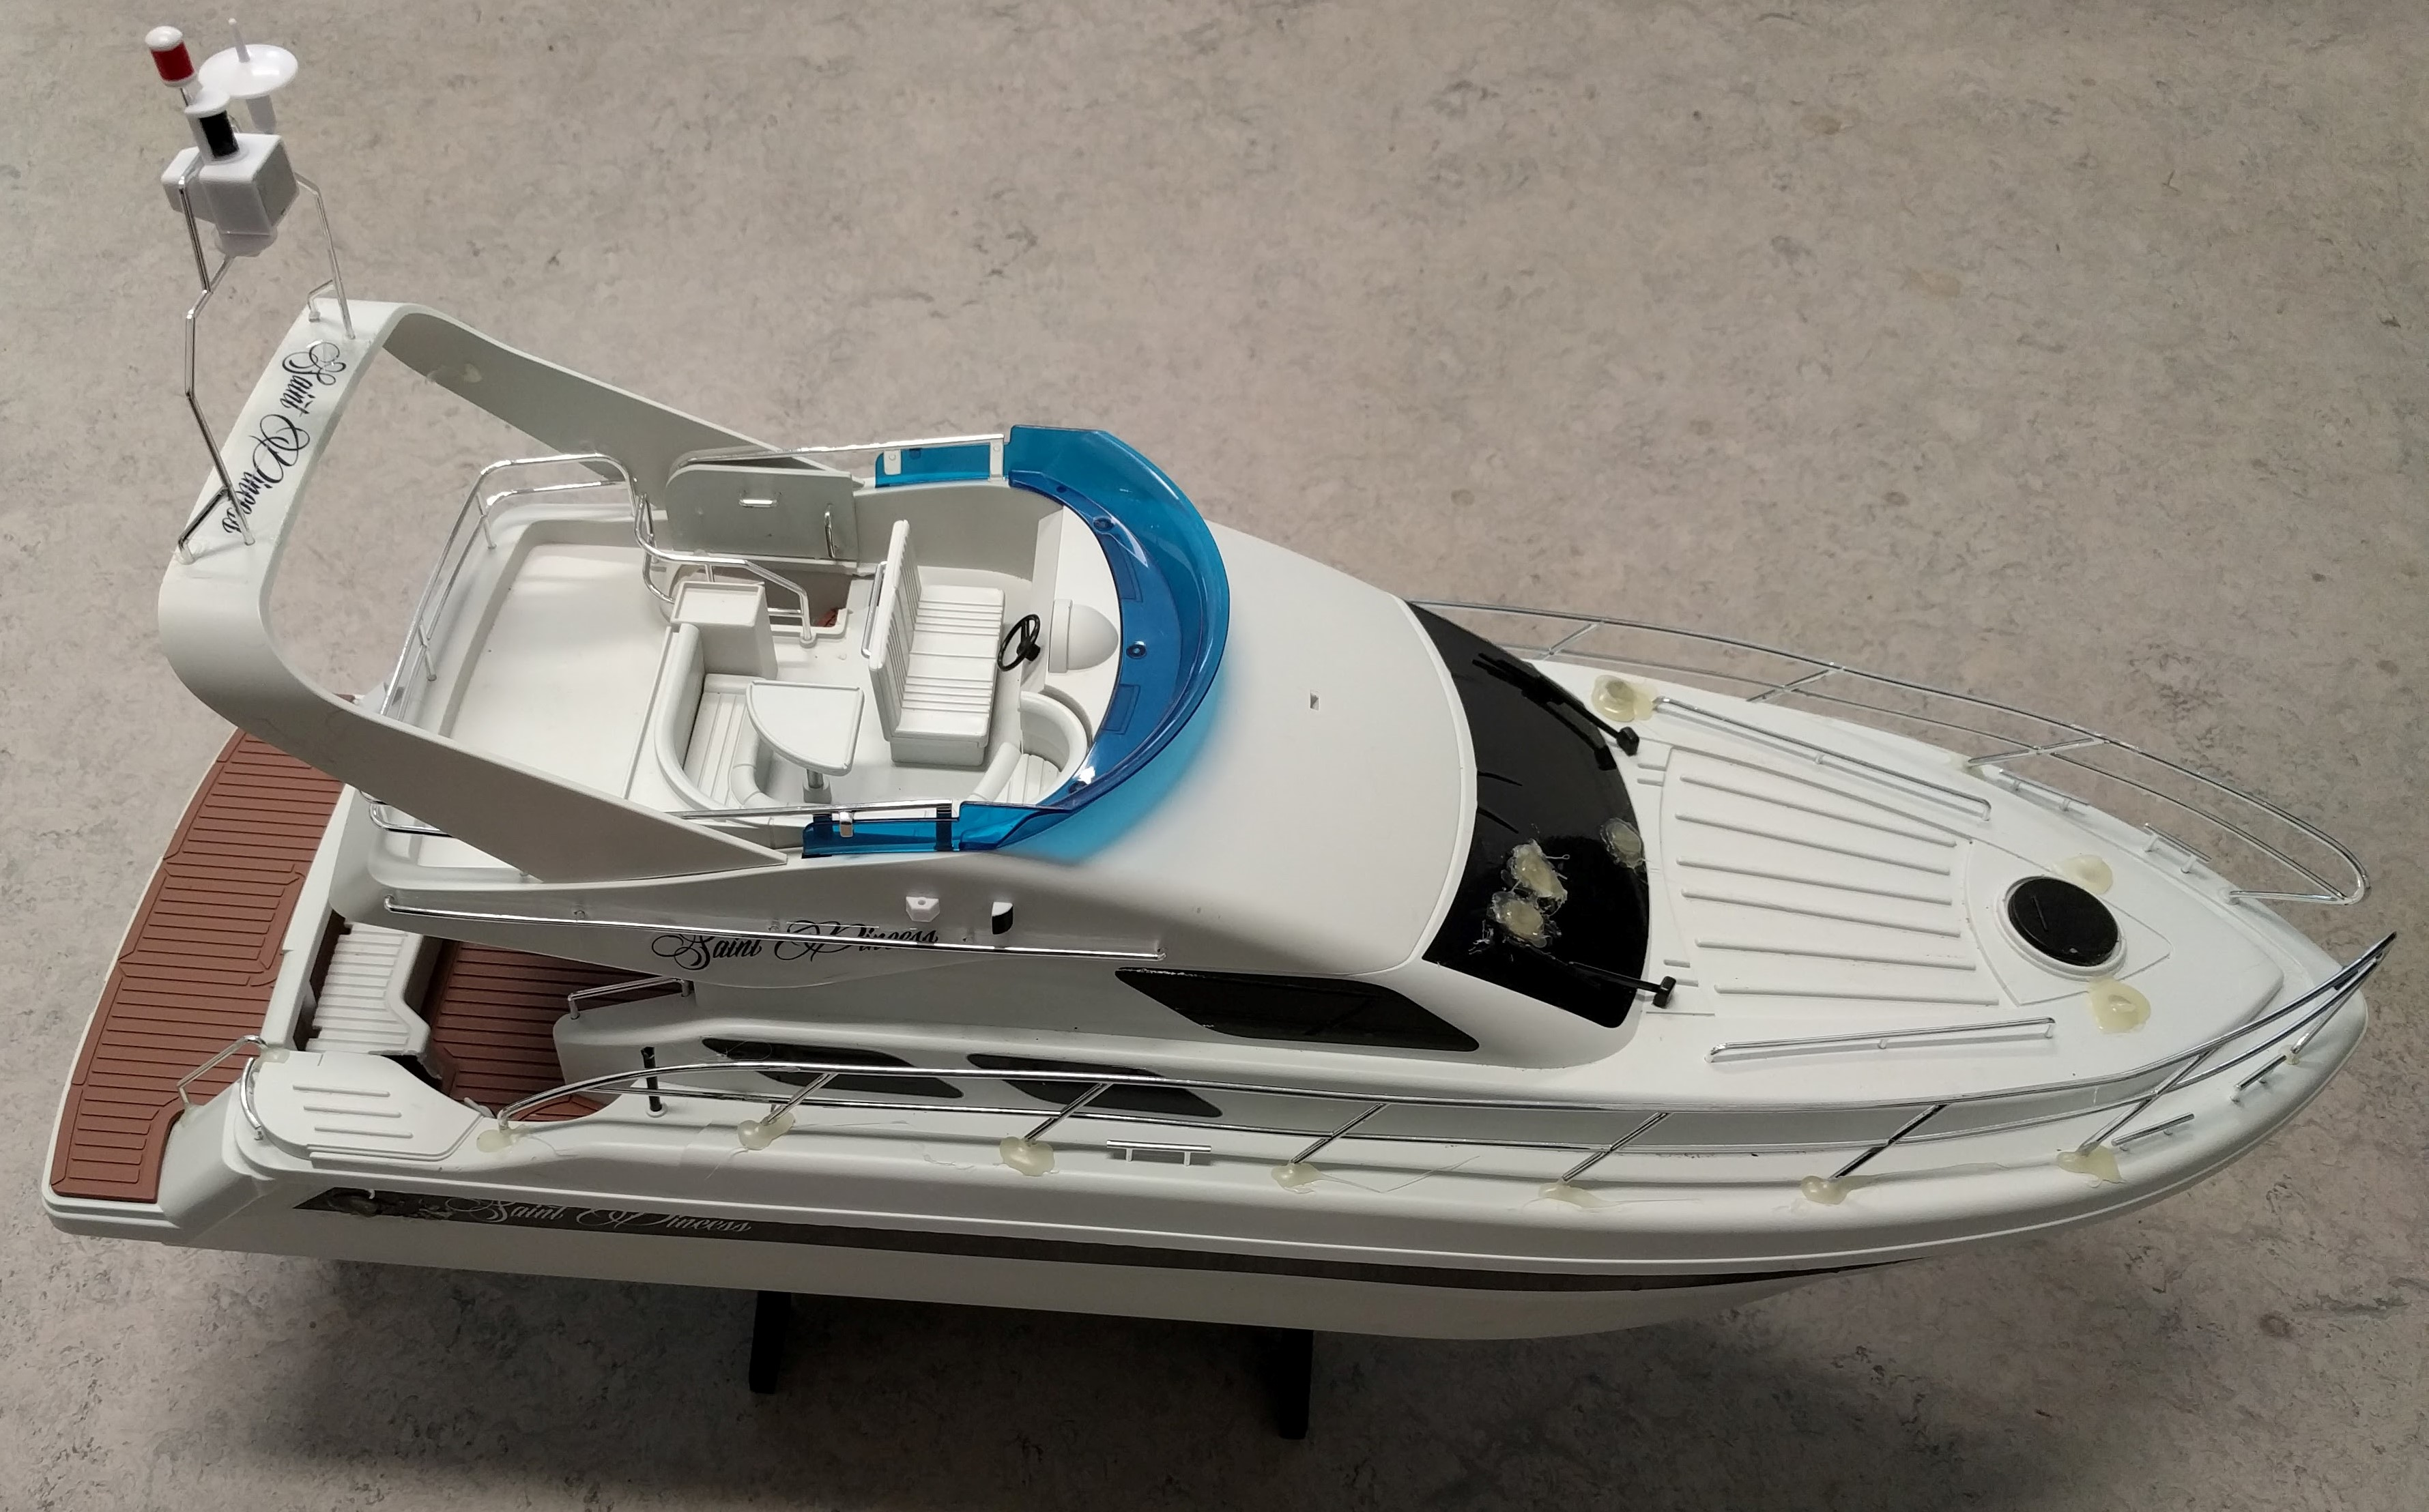
\includegraphics[width=0.7\linewidth]{Images/Implementation/boat_hardware_enclosed}
\caption{Closed up boat with electronics inside}
\label{fig:boat_closed}
\end{figure}






%DC-DC
%%Servo
%%Rpi

%Servo

%Motor Controller

%Motor

%Level converter

%RPI connection

%GPS